%======================================================================
% University of Waterloo Thesis Template for LaTeX 
% Last Updated August 21, 2018 
% by Stephen Carr, IST Client Services, 
% University of Waterloo, 200 University Ave. W., Waterloo, Ontario, Canada
% FOR ASSISTANCE, please send mail to rt-IST-CSmathsci@rt.uwaterloo.ca

% DISCLAIMER
% To the best of our knowledge, this template satisfies the current uWaterloo thesis requirements.
% However, it is your responsibility to assure that you have met all 
% requirements of the University and your particular department.

% Many thanks for the feedback from many graduates who assisted the development of this template.
% Also note that there are explanatory comments and tips throughout this template.
%======================================================================
% Some important notes on using this template and making it your own...

% The University of Waterloo has required electronic thesis submission since October 2006. 
% See the uWaterloo thesis regulations at
% https://uwaterloo.ca/graduate-studies/thesis.
% This thesis template is geared towards generating a PDF 
% version optimized for viewing on an electronic display, including 
% hyperlinks within the PDF.

% DON'T FORGET TO ADD YOUR OWN NAME AND TITLE in the "hyperref" package
% configuration below. THIS INFORMATION GETS EMBEDDED IN THE PDF FINAL PDF DOCUMENT.
% You can view the information if you view properties of the PDF document.

% Many faculties/departments also require one or more printed
% copies. This template attempts to satisfy both types of output. See additional notes below.
% It is based on the standard "book" document class which provides all necessary 
% sectioning structures and allows multi-part theses.

% If you are using this template in Overleaf (cloud-based collaboration service), then it is 
% automatically processed and previewed for you as you edit.

% For people who prefer to install their own LaTeX distributions on their own computers, and process 
% the source files manually, the following notes provide the sequence of tasks:
 
% E.g. to process a thesis called "mythesis.tex" based on this template, run:

% pdflatex mythesis	-- first pass of the pdflatex processor
% bibtex mythesis	-- generates bibliography from .bib data file(s)
% makeindex         -- should be run only if an index is used 
% pdflatex mythesis	-- fixes numbering in cross-references, bibliographic references, glossaries, index, etc.
% pdflatex mythesis	-- it takes a couple of passes to completely process all cross-references

% If you use the recommended LaTeX editor, Texmaker, you would open the mythesis.tex
% file, then click the PDFLaTeX button. Then run BibTeX (under the Tools menu).
% Then click the PDFLaTeX button two more times. If you have an index as well,
% you'll need to run MakeIndex from the Tools menu as well, before running pdflatex
% the last two times.

% N.B. The "pdftex" program allows graphics in the following formats to be
% included with the "\includegraphics" command: PNG, PDF, JPEG, TIFF
% Tip 1: Generate your figures and photos in the size you want them to appear
% in your thesis, rather than scaling them with \includegraphics options.
% Tip 2: Any drawings you do should be in scalable vector graphic formats:
% SVG, PNG, WMF, EPS and then converted to PNG or PDF, so they are scalable in
% the final PDF as well.
% Tip 3: Photographs should be cropped and compressed so as not to be too large.

% To create a PDF output that is optimized for double-sided printing: 
%
% 1) comment-out the \documentclass statement in the preamble below, and
% un-comment the second \documentclass line.
%
% 2) change the value assigned below to the boolean variable
% "PrintVersion" from "false" to "true".

%======================================================================
%   D O C U M E N T   P R E A M B L E
% Specify the document class, default style attributes, and page dimensions, etc.
% For hyperlinked PDF, suitable for viewing on a computer, use this:
\documentclass[A4paper,12pt,titlepage,oneside,final]{book}
 
% For PDF, suitable for double-sided printing, change the PrintVersion variable below
% to "true" and use this \documentclass line instead of the one above:
%\documentclass[letterpaper,12pt,titlepage,openright,twoside,final]{book}
%\documentclass[A4paper,12pt,titlepage,openright,twoside,final]{book}

% Some LaTeX commands I define for my own nomenclature.
% If you have to, it's easier to make changes to nomenclature once here than in a 
% million places throughout your thesis!
\newcommand{\package}[1]{\textbf{#1}} % package names in bold text
\newcommand{\cmmd}[1]{\textbackslash\texttt{#1}} % command name in tt font 
\newcommand{\href}[1]{#1} % does nothing, but defines the command so the
    % print-optimized version will ignore \href tags (redefined by hyperref pkg).
%\newcommand{\texorpdfstring}[2]{#1} % does nothing, but defines the command
% Anything defined here may be redefined by packages added below...

% This package allows if-then-else control structures.
\usepackage{ifthen}
\newboolean{PrintVersion}
\setboolean{PrintVersion}{false}
% CHANGE THIS VALUE TO "true" as necessary, to improve printed results for hard copies
% by overriding some options of the hyperref package, called below.

%\usepackage{nomencl} % For a nomenclature (optional; available from ctan.org)
\usepackage{amsmath,amssymb,amstext} % Lots of math symbols and environments
\usepackage[pdftex]{graphicx} % For including graphics N.B. pdftex graphics driver 

% Hyperlinks make it very easy to navigate an electronic document.
% In addition, this is where you should specify the thesis title
% and author as they appear in the properties of the PDF document.
% Use the "hyperref" package 
% N.B. HYPERREF MUST BE THE LAST PACKAGE LOADED; ADD ADDITIONAL PKGS ABOVE
\usepackage[pdftex,pagebackref=false]{hyperref} % with basic options
%\usepackage[pdftex,pagebackref=true]{hyperref}
		% N.B. pagebackref=true provides links back from the References to the body text. This can cause trouble for printing.
\hypersetup{
    plainpages=false,       % needed if Roman numbers in frontpages
    unicode=false,          % non-Latin characters in Acrobat’s bookmarks
    pdftoolbar=true,        % show Acrobat’s toolbar?
    pdfmenubar=true,        % show Acrobat’s menu?
    pdffitwindow=false,     % window fit to page when opened
    pdfstartview={FitH},    % fits the width of the page to the window
%    pdftitle={uWaterloo\ LaTeX\ Thesis\ Template},    % title: CHANGE THIS TEXT!
%    pdfauthor={Author},    % author: CHANGE THIS TEXT! and uncomment this line
%    pdfsubject={Subject},  % subject: CHANGE THIS TEXT! and uncomment this line
%    pdfkeywords={keyword1} {key2} {key3}, % list of keywords, and uncomment this line if desired
    pdfnewwindow=true,      % links in new window
    colorlinks=true,        % false: boxed links; true: colored links
    linkcolor=blue,         % color of internal links
    citecolor=green,        % color of links to bibliography
    filecolor=magenta,      % color of file links
    urlcolor=cyan           % color of external links
}
\ifthenelse{\boolean{PrintVersion}}{   % for improved print quality, change some hyperref options
\hypersetup{	% override some previously defined hyperref options
%    colorlinks,%
    citecolor=black,%
    filecolor=black,%
    linkcolor=black,%
    urlcolor=black}
}{} % end of ifthenelse (no else)

\usepackage[automake,toc,abbreviations]{glossaries-extra} % Exception to the rule of hyperref being the last add-on package
% If glossaries-extra is not in your LaTeX distribution, get it from CTAN (http://ctan.org/pkg/glossaries-extra), 
% although it's supposed to be in both the TeX Live and MikTeX distributions. There are also documentation and 
% installation instructions there.
\usepackage{caption}
\usepackage{subcaption}
\usepackage{mathrsfs}
\usepackage{amsmath}
\usepackage{amssymb}
\usepackage{array}
\usepackage{graphicx,rotating,booktabs}
\usepackage[verbose]{placeins}
%\usepackage[ngerman]{babel}
\usepackage{blindtext}
\usepackage{multirow}

% Setting up the page margins...
% uWaterloo thesis requirements specify a minimum of 1 inch (72pt) margin at the
% top, bottom, and outside page edges and a 1.125 in. (81pt) gutter
% margin (on binding side). While this is not an issue for electronic
% viewing, a PDF may be printed, and so we have the same page layout for
% both printed and electronic versions, we leave the gutter margin in.
% Set margins to minimum permitted by uWaterloo thesis regulations:
\setlength{\marginparwidth}{0pt} % width of margin notes
% N.B. If margin notes are used, you must adjust \textwidth, \marginparwidth
% and \marginparsep so that the space left between the margin notes and page
% edge is less than 15 mm (0.6 in.)
\setlength{\marginparsep}{0pt} % width of space between body text and margin notes
\setlength{\evensidemargin}{0.125in} % Adds 1/8 in. to binding side of all 
% even-numbered pages when the "twoside" printing option is selected
\setlength{\oddsidemargin}{0.125in} % Adds 1/8 in. to the left of all pages
% when "oneside" printing is selected, and to the left of all odd-numbered
% pages when "twoside" printing is selected
\setlength{\textwidth}{6.375in} % assuming US letter paper (8.5 in. x 11 in.) and 
% side margins as above
\raggedbottom

% The following statement specifies the amount of space between
% paragraphs. Other reasonable specifications are \bigskipamount and \smallskipamount.
\setlength{\parskip}{\medskipamount}

% The following statement controls the line spacing.  The default
% spacing corresponds to good typographic conventions and only slight
% changes (e.g., perhaps "1.2"), if any, should be made.
\renewcommand{\baselinestretch}{1} % this is the default line space setting

% By default, each chapter will start on a recto (right-hand side)
% page.  We also force each section of the front pages to start on 
% a recto page by inserting \cleardoublepage commands.
% In many cases, this will require that the verso (left-hand) page be
% blank, and while it should be counted, a page number should not be
% printed.  The following statements ensure a page number is not
% printed on an otherwise blank verso page.
\let\origdoublepage\cleardoublepage
\newcommand{\clearemptydoublepage}{%
  \clearpage{\pagestyle{empty}\origdoublepage}}
\let\cleardoublepage\clearemptydoublepage

% Define Glossary terms (This is properly done here, in the preamble and could also be \input{} from a separate file...)
% Main glossary entries -- definitions of relevant terminology
\newglossaryentry{computer}
{
name=computer,
description={A programmable machine that receives input data,
               stores and manipulates the data, and provides
               formatted output}
}

% Nomenclature glossary entries -- New definitions, or unusual terminology
\newglossary*{nomenclature}{Nomenclature}
\newglossaryentry{dingledorf}
{
type=nomenclature,
name=dingledorf,
description={A person of supposed average intelligence who makes incredibly brainless misjudgments}
}

% List of Abbreviations (abbreviations type is built in to the glossaries-extra package)
\newabbreviation{aaaaz}{AAAAZ}{American Association of Amateur Astronomers and Zoologists}

% List of Symbols
\newglossary*{symbols}{List of Symbols}
\newglossaryentry{rvec}
{
name={$\mathbf{v}$},
sort={label},
type=symbols,
description={Random vector: a location in n-dimensional Cartesian space, where each dimensional component is determined by a random process}
}
 
\makeglossaries

%======================================================================
%   L O G I C A L    D O C U M E N T
% The logical document contains the main content of your thesis.
% Being a large document, it is a good idea to divide your thesis
% into several files, each one containing one chapter or other significant 
% chunk of content, so you can easily shuffle things around later if desired.
%======================================================================
\begin{document}

%----------------------------------------------------------------------
% FRONT MATERIAL
% title page,declaration, borrowers' page, abstract, acknowledgements,
% dedication, table of contents, list of tables, list of figures, nomenclature, etc.
%----------------------------------------------------------------------
% T I T L E   P A G E
% -------------------
% Last updated June 14, 2017, by Stephen Carr, IST-Client Services
% The title page is counted as page `i' but we need to suppress the
% page number. Also, we don't want any headers or footers.
\pagestyle{empty}
\pagenumbering{roman}

% The contents of the title page are specified in the "titlepage"
% environment.
\begin{titlepage}
        \begin{center}
        \vspace*{1.0cm}

        \Huge
        {\bf A No-Reference Method for Assessing the Quality of Multiply-Distorted Images}

        \vspace*{1.0cm}

        \normalsize
        by \\

        \vspace*{1.0cm}

        \Large
        Pooryaa Cheraaqee \\

        \vspace*{3.0cm}

        \normalsize
        A thesis \\
        presented to Kharazmi University \\ 
        in fulfillment of the \\
        thesis requirement for the degree of \\
        Masters of Science \\
        in \\
        Computer Engineering-Artificial Intelligence and Robotics \\

        \vspace*{2.0cm}

        Tehran, Tehran, Iran, 2019 \\

        \vspace*{1.0cm}

        %\copyright\ Pat Neugraad 2017 \\
        \end{center}
\end{titlepage}

% The rest of the front pages should contain no headers and be numbered using Roman numerals starting with `ii'
\pagestyle{plain}
\setcounter{page}{2}

\cleardoublepage % Ends the current page and causes all figures and tables that have so far appeared in the input to be printed.
% In a two-sided printing style, it also makes the next page a right-hand (odd-numbered) page, producing a blank page if necessary.

 
% E X A M I N I N G   C O M M I T T E E (Required for Ph.D. theses only)
% Remove or comment out the lines below to remove this page
\begin{center}\textbf{Examining Committee Membership}\end{center}
  \noindent
The following served on the Examining Committee for this thesis.
  \bigskip
  
  \noindent
\begin{tabbing}
Internal-External Member: \=  \kill % using longest text to define tab length
External Examiner: \>  Farah Torkamani Azar \\ 
\> Associate Professor, \\ \>Dept. of Telecommunication, \\ \>Shahid Beheshti University \\
\end{tabbing} 
  \bigskip
 \noindent
  \begin{tabbing}
Internal-External Member: \=  \kill % using longest text to define tab length
Internal Examiner: \> Manoochehr Kelarestaghi \\
\> Assistant Professor, \\ \>Dept. of Electrical and Computer Engineering, \\ \>Kharazmi University \\
\end{tabbing}
  \bigskip
  
  \noindent
\begin{tabbing}
Internal-External Member: \=  \kill % using longest text to define tab length
Supervisors: \> Azadeh Mansouri \\
\> Assistant Professor, \\ \>Dept. of Electrical and Computer Engineering,\\ \> Kharazmi University \\ \\
\> Ahmad Mahmoudi-Aznaveh \\
\> Assistant Professor, \\ \>Cyberspace Research Institute,\\ \> Shahid Beheshti University \\
\end{tabbing}
%  \bigskip
  
  
  
%  \noindent
%\begin{tabbing}
%Internal-External Member: \=  \kill % using longest text to define tab length
%Internal-External Member: \> Deepa Thotta \\
%\> Professor, Dept. of Philosophy, University of Waterloo \\
%\end{tabbing}
%  \bigskip
%  
%  \noindent
%\begin{tabbing}
%Internal-External Member: \=  \kill % using longest text to define tab length
%Other Member(s): \> Leeping Fang \\
%\> Professor, Dept. of Fine Art, University of Waterloo \\
%\end{tabbing}
%
\cleardoublepage

% D E C L A R A T I O N   P A G E
% -------------------------------
  % The following is a sample Delaration Page as provided by the GSO
  % December 13th, 2006.  It is designed for an electronic thesis.
  \noindent
This document is prepared using the thesis template available on https://www.overleaf.com/.

\cleardoublepage

% A B S T R A C T
% ---------------

\begin{center}\textbf{Abstract}\end{center}

Assessing the visual quality of digital images is of great importance, since humans are the typical users of multimedia applications, and their satisfaction is dependent on the perceived quality. Mathematical models of human-quality perception are desirable, since they can automate the monitoring and optimization of such services. However, the non-linear and complex human visual system is difficult to simulate, and machine learning methods are leveraged to predict human judgements on image quality. The existence of multiple distortions increases the complexity of assessment in comparison to the case of single distortions. To supply academic and practical demands, several datasets are provided for training and evaluation of multiple-distortion quality metrics. In this dissertation, a full-reference and a no-reference method are proposed for assessing multiply-distorted images that incorporate gradient orientations for representing micro structures. Experiments show that the generality of the proposed features is superior to the existing descriptors. The method is also shown to have an acceptable time complexity while being competitively accurate.

\cleardoublepage

% A C K N O W L E D G E M E N T S
% -------------------------------

\begin{center}\textbf{Acknowledgements}\end{center}

I would like to thank Dr. Mansouri, Dr. Mahmoudi-Aznaveh, my father, my mother, and my brother, for making this research possible.

I also thank Mohammad Minouei, Hossein Motamednia, Mojtaba Barekati, and Mohammad Ali Arghavan for sharing their creative ideas with me.
\cleardoublepage

% D E D I C A T I O N
% -------------------

%\begin{center}\textbf{Dedication}\end{center}

%This is dedicated to the one I love.
%\cleardoublepage

% T A B L E   O F   C O N T E N T S
% ---------------------------------
\renewcommand\contentsname{Table of Contents}
\tableofcontents
\cleardoublepage
\phantomsection    % allows hyperref to link to the correct page

% L I S T   O F   T A B L E S
% ---------------------------
\addcontentsline{toc}{chapter}{List of Tables}
\listoftables
\cleardoublepage
\phantomsection		% allows hyperref to link to the correct page

% L I S T   O F   F I G U R E S
% -----------------------------
\addcontentsline{toc}{chapter}{List of Figures}
\listoffigures
\cleardoublepage
\phantomsection		% allows hyperref to link to the correct page

% GLOSSARIES (Lists of definitions, abbreviations, symbols, etc. provided by the glossaries-extra package)
% -----------------------------
%\printglossaries
%\cleardoublepage
%\phantomsection		% allows hyperref to link to the correct page

% Change page numbering back to Arabic numerals
\pagenumbering{arabic}

 

%----------------------------------------------------------------------
% MAIN BODY
% We suggest using a separate file for each chapter of your thesis.
% Start each chapter file with the \chapter command.
% Only use \documentclass or \begin{document} and \end{document} commands 
% in this master document.
% Tip 4: Putting each sentence on a new line is a way to simplify later editing.
%----------------------------------------------------------------------
%======================================================================
\chapter{Introduction}
%======================================================================

Digital images are an important means for sharing information in the age of communication. Watching television or viewing images on smartphones are part of our daily lives and video accounts for a large portion data traffic~\cite{del}. Digital images are captured, synthesized, and shared for educational, recreational, or business purposes.

It is unpleasant for users to view a low-quality image and it is necessary in many situations to be provided with a measurement of image quality. For example, content providers are willing to be aware of the quality of images viewed by their users and detect the defected pictures. The process of image acquisition can also repeat, until a satisfactory quality is achieved. Compression algorithms try to reduce the size of images, while maintaining its quality. Reduction of size is obtained with loss of information which is followed by image distortion. Therefore, with measuring the quality of the compressed image, the trade off between size and quality can be optimized.

The straight-forward way to evaluate the quality of an image, is to survey human opinions~\cite{Ghadiyaram2016}. A set of subjects view the image and each of them gives a score to the quality of the image. The average of these scores, called \emph{mean opinion score}-MOS, is a reliable measurement of the visual quality of the test picture.

The process described above, is called subjective assessment and it is infeasible for online, large-scale or real-time applications. Hence, automatic methods are desirable that can predict human's judgement on the quality of an image. However, due to its complexity, human visual system (HVS) is difficult to model and the prediction of an algorithm may not be well correlated with the opinion of human.

Devising computational models that can correctly predict human opinion on the quality of a digital picture, is called objective image quality assessment (IQA). The accuracy and speed of this prediction are the performance criteria of a proposed algorithm. The accuracy of a method is measured by the correlation between its scores and the scores obtained from subjective assessments.

In this thesis, the problem of objective IQA is studied. I the following sections a classification of the problem and an introduction on multiple distortions is presented.

\section{Classes of Objective IQA Problems}
According to the availability of a pristine image, there can be three cases when evaluating the quality of a distorted picture. In some scenarios, like image compression, a distorted version of the original image is produced by the compression algorithm. So when assessing the quality of the compressed image, the original can be used as a reference. This case is called \emph{full reference}-FR IQA. If instead of pixel-by-pixel values, there are some information available from the reference image, like an extracted feature vector, the assessment is called \emph{reduced reference}-RR IQA. This case can happen in image communications when it is expensive and unreliable to transmit bulky images.

An example for the case that there are no reference images, is a hand-held camera that captures multiple shots at a time and automatically selects the one with highest visual quality. There are no references available from the recorded scene and the evaluation must be done in a \emph{no reference}-NR manner. It is obvious that correct prediction in NR IQA is more difficult~\cite{Kang2014}.

Although IQA methods can be classified in different ways, but we will have the least overlap when classifying according to the availability of a reference picture. However, there are methods that can be adapted to a desirable amount of information from a reference signal~\cite{Bosse2018, torkamani2018image}. In this research, a FR and a NR objective IQA methods are proposed and evaluated.
%----------------------------------------------
\section{Distortions in an Image}
%----------------------------------------------
Common distortions that cause deviation in the perceived quality of images, are limited in practice~\cite{Chandler2013}. Blocking effect, out-of-focus blur, and white Gaussian noise are examples of these artifacts. If we are already aware of the distortion type that contaminated the image and we want to measure its severity, we are performing a \emph{distortion-specific} assessment. \emph{General-purpose} or \emph{non-distortion-specific} assessment, addresses the case that the image can be distorted with an arbitrary artifact and the algorithm is not aware of its type.

There has been numerous studies for distortion-specific and general-purpose IQA~\cite{lin2010perceptual, Chikkerur2011, xu2017no, Manap2015, borse2014competitive} and many datasets of distorted images are available along with their corresponding subjective scores~\cite{Sheikh,Chandler2010,Ponomarenko2015,Ponomarenko2009,Horita}. Each distorted image in these datasets is contaminated with one type of distortions of arbitrary severity, i.e., the image is \emph{singly-distorted}.

In real-world problems, an image can have multiple distortions. An example is an image that is blurred because of environmental conditions at the time of acquisition, and then quantized by compression, and noised after transmission. In 2012, Jayaraman et al.~\cite{Jayaraman2012}, provided a dataset of subject-rated \emph{multiply-distorted} images and demonstrated that the accuracy of methods devised for single distortions, drops significantly when applied to multiply-distorted images. Therefore, different approaches are required for multiple distortions~\cite{Li2016}.

With the increase in academic and commercial demands, two other datasets are constructed for training and testing the algorithms on multiply-distorted images~\cite{Sun2017, Gu2014} and many current IQA studies are devoted to multiple distortions~\cite{Li2016,Gu2014,Dai2018,Chetouani2016,Chetouani2015,Li2018a,Mahmoudpour2018,Mahmoudpour2017,Gu2013,miao2019quality,wang2019blind, zhang2019full, lu2015no}. IQA of multiply-distorted images is the problem that is tackled in this thesis.
%---------------------------------------------------------------------
\section{Objectives and Motivations}
%---------------------------------------------------------------------
Many image processing systems lack a reliable and fast metric of image quality. Parameters related to contrast and luminance of hand-held digital cameras can be automatically set for any arbitrary scene according to a measure of quality~\cite{Alakarhu2007}. Compression algorithms can also optimize the quantization using the metric~\cite{Zhai2008,Zhang2011}. Another example is video streaming services in which, streaming resources can be allocated in a smarter manner according to the quality of the videos~\cite{Anegekuh2015}. Image recommendation systems can also sort the images based on a quality index~\cite{Gaur2014}.

Subjective assessments must be proceeded according to certain standards and comply certain conditions~\cite{VQEG2000}. For example, the number of subjects must satisfy the requirements for statistical reliability. Also, the display condition and the rating format affect the opinion of the participants. Regardless of the tediousness of subjective experiments, it is not possible to survey human judgements in on-line and real-time applications and automation is the only option in these cases. So, a fast and reliable image quality metric is of great practical interest.

Occurrence of multiple distortions in real-world problems demands methods that can handle the mutual and joint effect of the artifacts. On the other hand, traditional methods are greatly challenged in assessing the quality of multiply-distorted images.

These theoretical and practical necessities motivates us to study the objective assessment of multiple distortions. Since the eventual observer in the majority of image processing applications is the human~\cite{Ghadiyaram2016}, the intelligence of an objective IQA system is measured by its ability to mimic human rating and we aim to propose a metric with an acceptable performance on subject-rated multiply-distorted IQA datasets.

In this chapter, we introduced and classified the problem of objective IQA, mentioned its applications, and distinguished the cases of single and multiple distortions. In the rest of the thesis we review the literature in Chapter 2 and propose a FR and a NR method in Chapter 3. In Chapter 4 the method is tested and the thesis is concluded with suggestions for future studies.

%======================================================================
\chapter{Literature Review}
%======================================================================
For a long time (until 2002), mean squared error (MSE) and peak signal to noise ratio (PSNR) were the common criteria for comparing the quality of a distorted image to a reference~\cite{Wang2004}. Although these metrics are intuitively explainable and computationally efficient, they are not well-correlated with human opinions~\cite{Wang2009,Wang2002}. Structural similarity was proposed to cover this gap~\cite{Wang2002a}. With the introduction of this criterion, many methods were proposed to measure the structural similarity, which a large number of them are based on image edges~\cite{Xue2014}.

For referenceless assessment, natural scene statistics (NSS) were the criterion of choice for many metrics. Ruderman~\cite{Ruderman1994} showed that natural images\footnote{``An image recorded from the physical environment with a camera that is sensitive to the visible spectrum of electromagnetic wave"~\cite{Liu2014a}} obey statistical regularities that are stable, regardless of the image content. So deviation from these regularities were exploited as a measure for distortion.

With the introduction of multiple distortion datasets, methods were proposed that tried to consider the simultaneous existence of multiple distortions in an image and extract features that describe their severity.

In this chapter we introduce the structural similarity criterion and two methods for its measurement. Then we review the approaches taken for NR IQA. The FR, RR, and NR algorithms proposed for IQA of multiply-distorted images are explained and analyzed in subsequent sections.
%-------------------------------------------------------------------
\section{FR Methods for Single Distortion IQA}
%------------------------------------------------------------------
Numerous researches in IQA were conducted for full reference assessment~\cite{lin2010perceptual}. Assuming a reference image, $r$, and its distorted version, $d$; computing the difference between $r$ and $d$ maybe the first approach that comes to our minds for comparing them. This is what MSE, PSNR, or RMSE do. For two grayscale images, $r$ and $d$:
\begin{equation}
    MSE(r, d) = \frac{1}{M\times N}\sum_{x=1}^M\sum_{y=1}^N(r(x, y)-d(x, y))^2
    \label{eq:mse}
\end{equation}
Where $M$ and $N$ are image dimensions. For two identical images, MSE will be zero and this is in accordance with our opinion: \emph{`` the quality perceived from two identical images is the same"}, but there are many cases that MSE is independent of image distortions; Fig.~\ref{fig:einstein} shows an example (figure from~\cite{Wang2004}).
\begin{figure}
     \centering
     \begin{subfigure}[b]{0.3\textwidth}
         \centering
         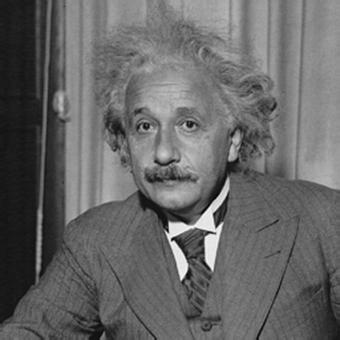
\includegraphics[width=\textwidth]{./figs/image003}
         \caption{Einstein's photo\\.\\.}
         \label{fig:einstein-orig}
     \end{subfigure}
     \hfill
     \begin{subfigure}[b]{0.3\textwidth}
         \centering
         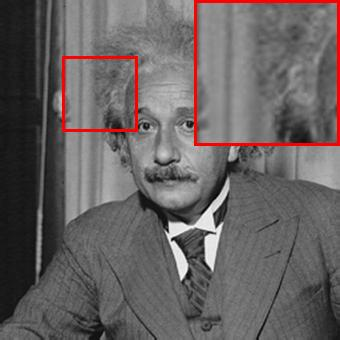
\includegraphics[width=\textwidth]{./figs/image003_bn}
         \caption{original image\\$MSE=0$\\$SSIM=1$}
         \label{fig:einstein-orig-s}
     \end{subfigure}
     \hfill
     \begin{subfigure}[b]{0.3\textwidth}
         \centering
         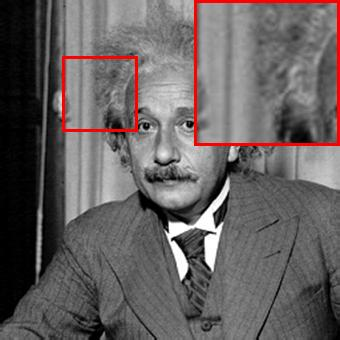
\includegraphics[width=\textwidth]{./figs/image0_bn}
         \caption{contrast change\\$MSE=144$\\$SSIM=0.913$}
         \label{fig:einstein-cc}
     \end{subfigure}
     \\
     \begin{subfigure}[b]{0.3\textwidth}
         \centering
         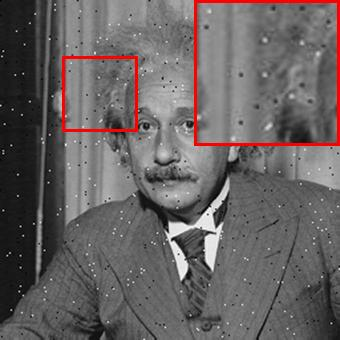
\includegraphics[width=\textwidth]{./figs/image009_bn}
         \caption{salt \& pepper noise\\$MSE=144$\\$SSIM=0.840$}
         \label{fig:einstein-sp}
     \end{subfigure}
     \hfill
     \begin{subfigure}[b]{0.3\textwidth}
         \centering
         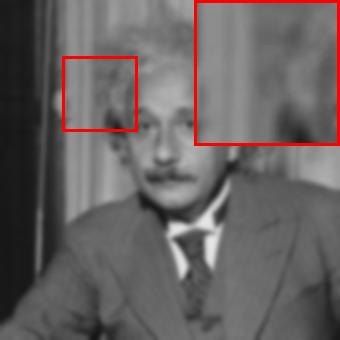
\includegraphics[width=\textwidth]{./figs/image011_bn}
         \caption{blur\\$MSE=144$\\$SSIM=0.694$}
         \label{fig:einstein-bl}
     \end{subfigure}
     \hfill
     \begin{subfigure}[b]{0.3\textwidth}
         \centering
         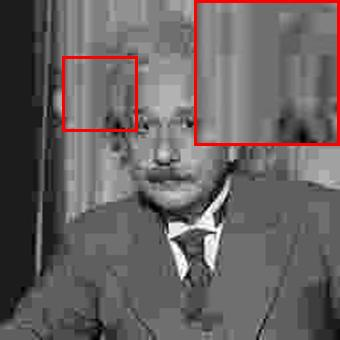
\includegraphics[width=\textwidth]{./figs/image013_bn}
         \caption{Jpeg quantization\\$MSE=144$\\$SSIM = 0.662$}
         \label{fig:einstein-jp}
     \end{subfigure}
        \caption{$MSE$ and $SSIM$ for different distorted versions of Einstein's photo.}
        \label{fig:einstein}
\end{figure}
We see different versions of the reference image in Fig.~\ref{fig:einstein-orig} with four artifacts ( the image in Fig.~\ref{fig:einstein-orig-s} is the reference, only magnified). MSE for the identical images equals zero (Fig.~\ref{fig:einstein-orig-s}), but in spite of the different visual quality of images in Fig.~\ref{fig:einstein-cc}-~\ref{fig:einstein-jp}, MSE is the same for all them, while a human observer prefers the image in Fig.~\ref{fig:einstein-cc} to the image in Fig.~\ref{fig:einstein-jp}.

MSE and similar approaches are based on ``error visibility". Wang and Bovik~\cite{Wang2002a} showed that the semantic information which we grasp from images are based on image structures. With a degradation in image structures we do not understand what we expect from a scene and perceive this as a low quality. They proposed a method, called `` SSIM~\cite{Wang2004}", for measuring the \underline{s}tructural \underline{sim}ilarity between two images. With the popularity of this method, researchers proposed other metrics for structural similarity and, as mentioned before, many of them are based on image edges. In what follows SSIM and one of the gradient based methods are explained.
%-------------------------------------------------------------------------------
\subsection{Structural Similarity}
%------------------------------------------------------------------------------
SSIM assumes that the structural similarity of two images is dependent on three factors: the correlation between the images, the luminance similarity, and the contrast similarity of the two image. That is, the more similar the two images are according to these criteria, the better is the quality of the distorted image. The abstract definition of SSIM for two grayscale images, $r$ and $d$, will be as follows:
\begin{eqnarray*}
\lefteqn{SSIM(r, d) = }\\
& & pixel\_wise\_correlation\times\\
& & luminance\_similarity\times\\
& & contrast\_similarity
\end{eqnarray*}
In SSIM, the contrast of an image is modeled with the variation in intensity values of pixels and luminance is modeled with the average of the values. If $I$ is an image with $N$ pixels, its luminance and contrast are represented as $\mu_I$ and $\sigma_I$, respectively, and obtained via the statistical definitions:
\begin{equation}
    \mu_I = \frac{1}{N}\sum_{x=1}^{N}I(x)
    \label{eq:mu}
\end{equation}
\begin{equation}
    \sigma_I = \sqrt{\frac{1}{N-1}\sum_{x=1}^N(I(x)-\mu_I)^2}
    \label{eq:sigma}
\end{equation}
Where, $I(x)$ is the value of the $x^{th}$ pixel of $I$. For obtaining the similarity of two numbers, authors used a similarity relation. The similarity of two numbers, $a$ and $b$, are represented as $sim(a, b, c)$, and defined as:
\begin{equation}
    sim(a, b, c) = \frac{2\times a\times b+c}{a^2+b^2+c}
    \label{eq:sim}
\end{equation}
Where $c$ is a constant for avoiding the instability of the fraction. Therefore, contrast and luminance similarity for $r$ and $d$ is obtained from~\ref{eq:c_sim} and~\ref{eq:l_sim}.
\begin{equation}
    contrast\_similarity(r,d)=sim(\sigma_r, \sigma_d, c)\in [0, 1]
    \label{eq:c_sim}
\end{equation}
\begin{equation}
    luminance\_similarity(r, d) = sim(\mu_r, \mu_d, c)\in [0, 1]
    \label{eq:l_sim}
\end{equation}
The correlation between two images are defined as the statistical correlation of the intensity values of the pictures. If $r(x)$ and $d(x)$ are the $x^{th}$ pixel from the $N$ pixels in $r$ and $d$, the correlation between $r$ and $d$ is obtained from the following equation:
\begin{equation}
    pixel\_wise\_correlation(r, d) = \frac{\frac{1}{N-1}\sum_{x=1}^N(r(x)-\mu_r)(d(x)-\mu_d)}{\sigma_r\times \sigma_d} \in [-1, 1]
    \label{eq:corr}
\end{equation}
For two identical images, SSIM will be equal to one. It is expected that it decreases with the deviation of the image. In Fig.~\ref{fig:einstein} we see that this occurs and SSIM distinguishes different perceived qualities. It must be mentioned that SSIM is computed for each corresponding $8\times 8$ window in the images and for pooling the scores of the windows into one score for the entire image, the SSIM values are averaged.
\subsection{Similarity of Gradient Magnitude}
Apart from SSIM, there are other metrics proposed for measuring the structural similarity. One of the approaches, is considering the edges of the image as a representative of image structures. Image gradients are known as good estimations of the edges~\cite{Gonzalez2008}. In location $(x, y)$ of image $I$, the gradient vector $\Vec{G}_I(x, y)$ has a horizontal and a vertical component, $g_h$ and $g_v$, respectively. The magnitude and direction of $\Vec{G}_I$ in $(x, y)$ are defined in relations~\ref{eq:gm} and~\ref{eq:gd} with respect to these components.
\begin{equation}
    GM_I(x, y) = \sqrt{g_v^2+g_h^2}
    \label{eq:gm}
\end{equation}
\begin{equation}
    GD_I(x, y) = tan^{-1}(\frac{g_v}{g_h})
    \label{eq:gd}
\end{equation}
The method GMSD~\cite{Xue2014} used $GM$ for measuring image distortions.
\begin{figure}
     \centering
     \begin{subfigure}[b]{0.3\textwidth}
         \centering
         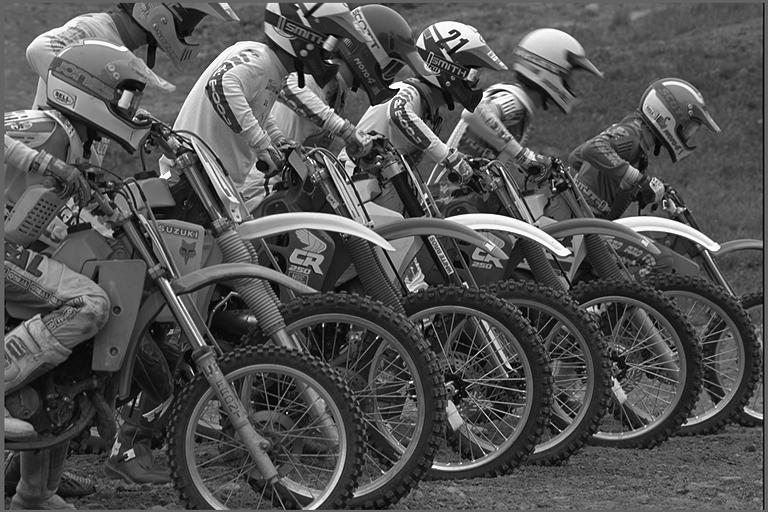
\includegraphics[width=\textwidth]{./figs/reference_gry}
         \caption{original image\\.}
         \label{fig:gmsd_ref_gry}
     \end{subfigure}
     \hfill
     \begin{subfigure}[b]{0.3\textwidth}
         \centering
         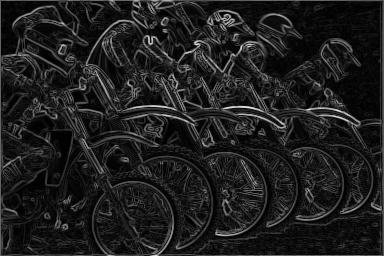
\includegraphics[width=\textwidth]{./figs/reference_mag}
         \caption{gradient magnitude of the original image}
         \label{fig:gmsd_ref_mag}
     \end{subfigure}
     \hfill
     \begin{subfigure}[b]{0.3\textwidth}
         \centering
         \fbox{
\includegraphics[width=0.9\textwidth]{./figs/reference_sim}}
         \caption{gradient magnitude similarity of the original image}
         \label{fig:gmsd_ref_sim}
     \end{subfigure}
     \\
     \begin{subfigure}[b]{0.3\textwidth}
         \centering
         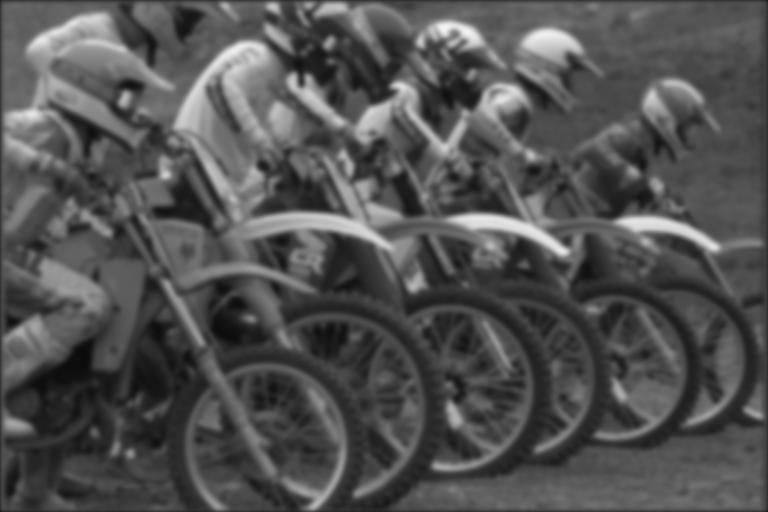
\includegraphics[width=\textwidth]{./figs/blur_gry}
         \caption{blurred image\\.}
         \label{fig:gmsd_blur_gry}
     \end{subfigure}
     \hfill
     \begin{subfigure}[b]{0.3\textwidth}
         \centering
         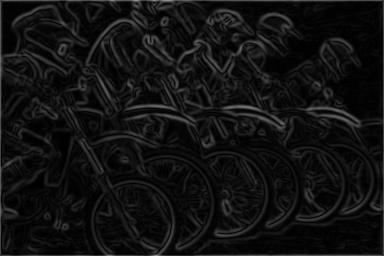
\includegraphics[width=\textwidth]{./figs/blur_mag}
         \caption{gradient magnitude of the blurred image}
         \label{fig:gmsd_blur_mag}
     \end{subfigure}
     \hfill
     \begin{subfigure}[b]{0.3\textwidth}
         \centering
         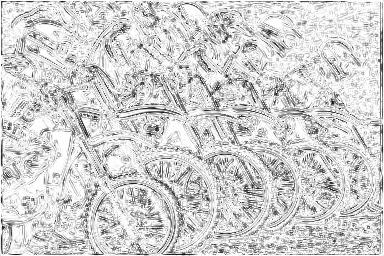
\includegraphics[width=\textwidth]{./figs/blur_sim}
         \caption{gradient magnitude similarity of the blurred image}
         \label{fig:gmsd_blur_sim}
     \end{subfigure}
     \\
     \begin{subfigure}[b]{0.3\textwidth}
         \centering
         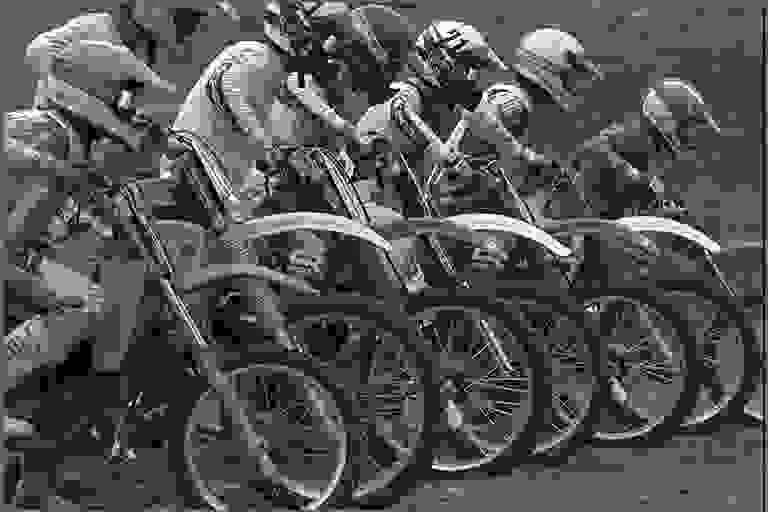
\includegraphics[width=\textwidth]{./figs/jpeg_gry}
         \caption{image with Jpeg artifact\\.}
         \label{fig:gmsd_jpeg_gry}
     \end{subfigure}
     \hfill
     \begin{subfigure}[b]{0.3\textwidth}
         \centering
         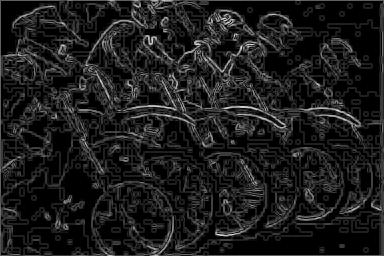
\includegraphics[width=\textwidth]{./figs/jpeg_mag}
         \caption{gradient magnitude of the Jpeg-compressed image}
         \label{fig:gmsd_jpeg_mag}
     \end{subfigure}
     \hfill
     \begin{subfigure}[b]{0.3\textwidth}
         \centering
         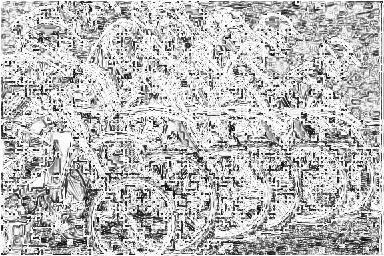
\includegraphics[width=\textwidth]{./figs/jpeg_sim}
         \caption{gradient magnitude similarity of the Jpeg image}
         \label{fig:gmsd_jpeg_sim}
     \end{subfigure}
     \\
     \begin{subfigure}[b]{0.3\textwidth}
         \centering
         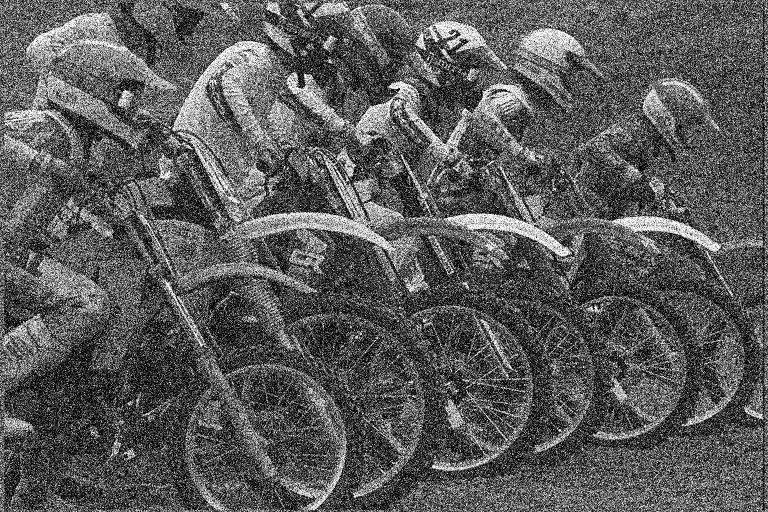
\includegraphics[width=\textwidth]{./figs/noise_gry}
         \caption{noisy image\\.}
         \label{fig:gmsd_noise_gry}
     \end{subfigure}
     \hfill
     \begin{subfigure}[b]{0.3\textwidth}
         \centering
         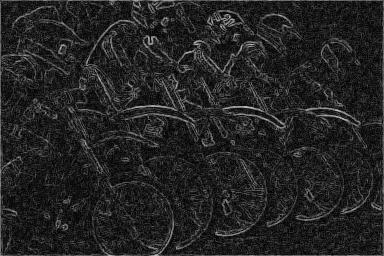
\includegraphics[width=\textwidth]{./figs/noise_mag}
         \caption{gradient magnitude of the noisy image}
         \label{fig:gmsd_noise_mag}
     \end{subfigure}
     \hfill
     \begin{subfigure}[b]{0.3\textwidth}
         \centering
         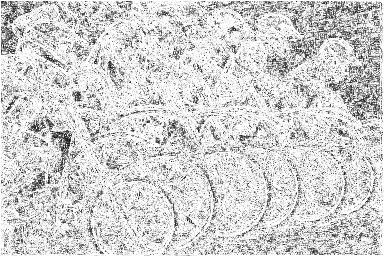
\includegraphics[width=\textwidth]{./figs/noise_sim}
         \caption{gradient magnitude similariy of the noisy image}
         \label{fig:gmsd_noise_sim}
     \end{subfigure}
        \caption{Different versions of an image with different distortions along with the gradient magnitude map and the map of gradient magnitude similarity with the original image.}
        \label{fig:gmsd}
\end{figure}
In Fig.~\ref{fig:gmsd} a sample is illustrated with its distorted versions and their gradient magnitudes. It is observable that image edges are sensitive to distortions. \underline{G}radient \underline{m}agnitude \underline{s}imilarity map for $r$ and $d$ is called $GMS(r, d)$ and defined as:
\begin{equation}
    GMS(r, d)_{(x, y)} = sim\left(GM_r(x, y), GM_d(x, y), c\right)
    \label{eq:gms}
\end{equation}
It is seen in Fig.~\ref{fig:gmsd_ref_sim} that GMS of an image and itself, equals to one for all pixels and when the image is degraded, this value will decrease (images in the right column).

GMSD computes the standard \underline{d}eviation for pooling the values of GMS. If $GMS(r, d)$ has $N$ pixels and $GMS(r, d)_x$ is the $x^{th}$ pixel, $GMSD(r, d)$ is obtained from the following equation:
\begin{equation}
    GMSD(r, d) = \sqrt{\frac{1}{N-1}\sum_{x=1}^{N}\left(GMS(r, d)_x-\frac{1}{N}\sum_{x=1}^NGMS(r, d)_x\right)^2}
\end{equation}
GMSD could improve the performance of SSIM, meanwhile, maintain a low computational complexity.

Considering image entropy~\cite{Sheikh2005, Sheikh2006}, different pooling strategies~\cite{Zhang2014a}, using image singular values~\cite{Mansouri2009, Mansouri2019}, analysis in wavelet domain~\cite{Chandler2007}, and taking color into account~\cite{Zhang2011a}, have been other innovations for FR IQA of singly distorted images.
%------------------------------------------------------------------------------------
\section{No-Reference IQA Methods}
%------------------------------------------------------------------------------------
The common approach of FR metrics is to define the quality score using mathematical relations~\cite{lin2010perceptual}. In the NR scenario, the distorted image is usually described with a feature vector and a model maps the vector to a quality score. This model can be a mathematical relation or be obtained using machine learning. The challenge for many NR IQA algorithms is to devise features that are expressive and fast to compute. Another strategy for feature extraction, is the use of machine learning techniques, such as \emph{convolutional neural networks-CNNs}. With CNNs, the feature vector can be achieved automatically. In what follows, the framework of \emph{feature-based} methods is presented, then the methods that are based on automatic feature extraction are reviewed.
\subsection{Feature-Based NR IQA Methods}
A common scheme for NR assessment, is extracting quality-relevant features. Then, with the use of machine learning methods, such as~\emph{support vector regression-SVR}, the features are mapped to quality scores. The required training data for machine learning can be obtained from the subjective scores in the image quality databases. The performance of these methods is dependent on the ability of the features to express the quality aspects of the image. The frameworks for training and testing of these methods is illustrated in Fig.~\ref{fig:svr_train} and Fig.~\ref{fig:svr_test}.
\begin{figure}
    \centering
    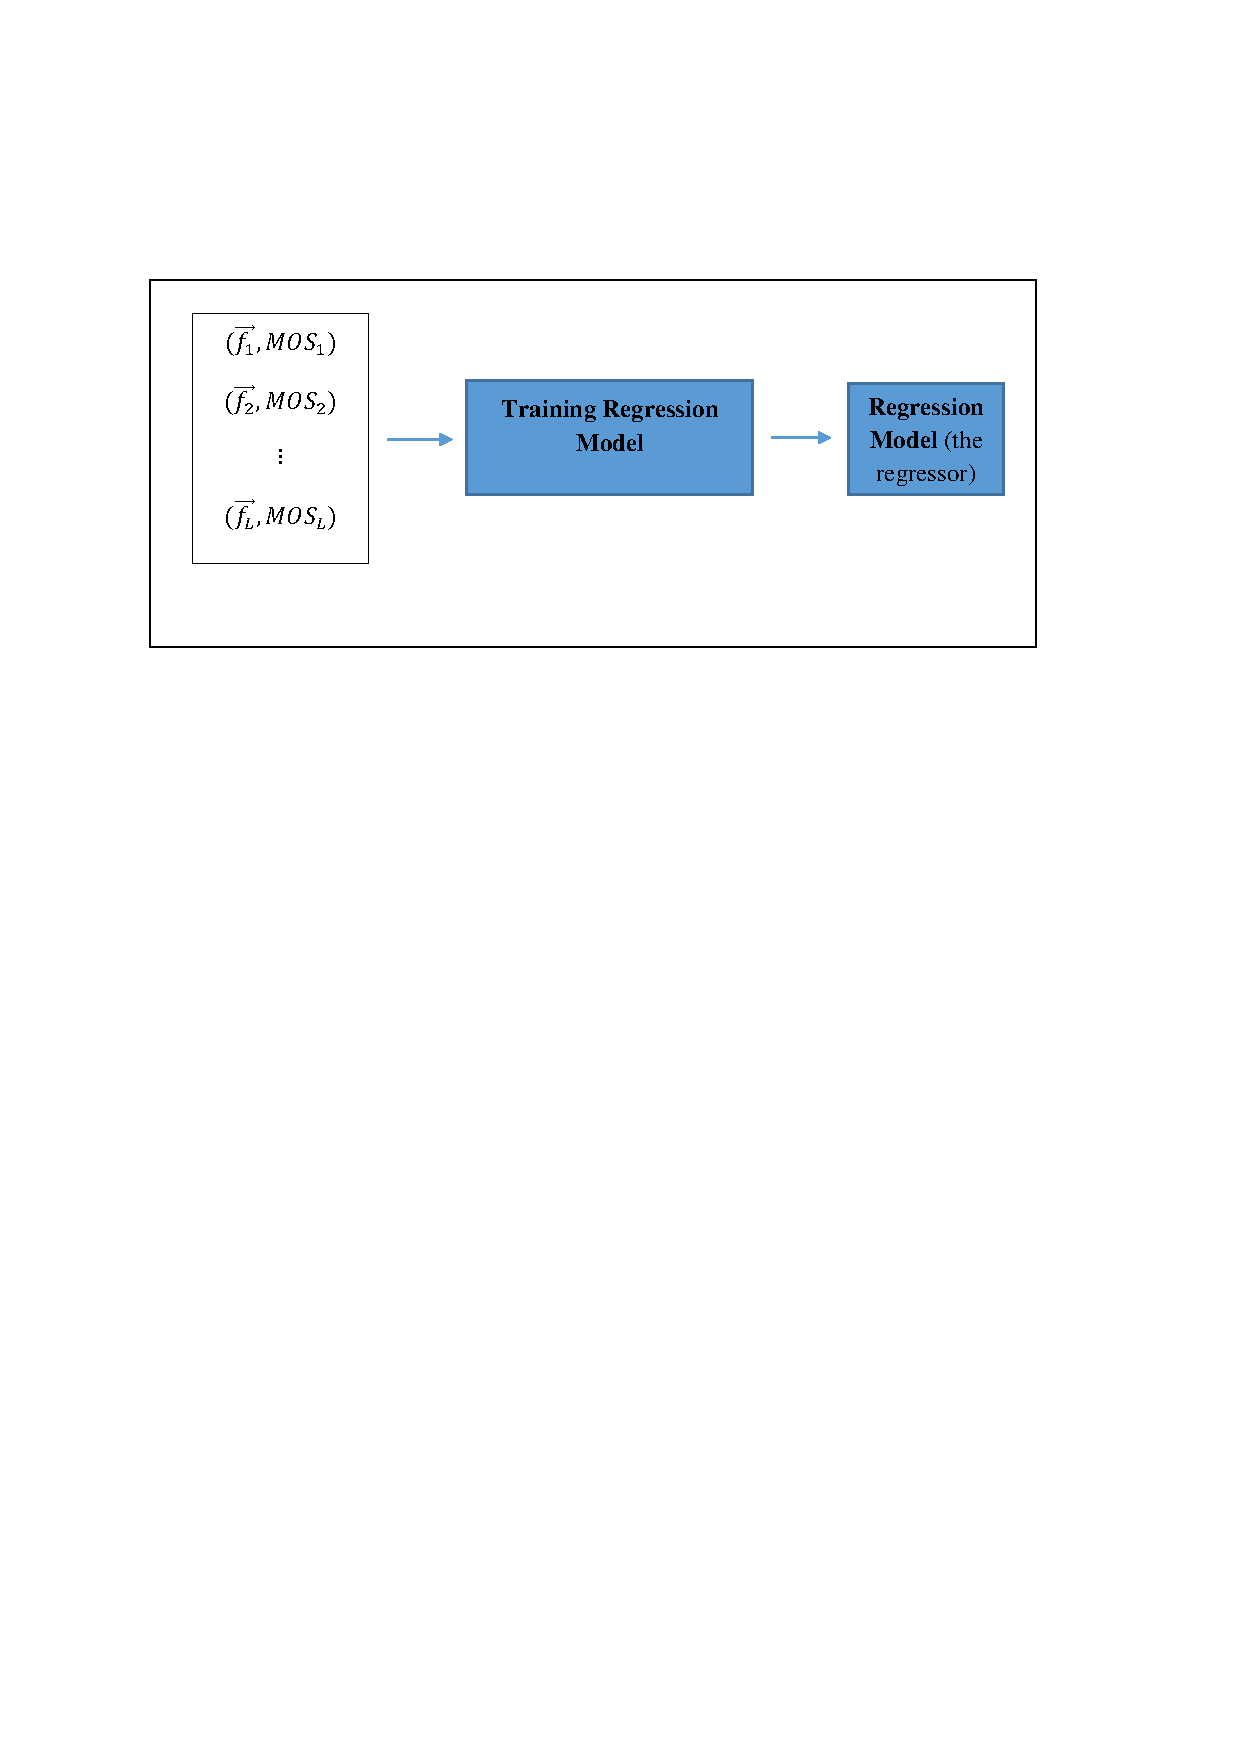
\includegraphics[width=\textwidth, trim={2.5cm 18.7cm 3.4cm 4.7cm}, clip]{./figs/fg_svr_train}
    \caption{Training feature-based methods}
    \label{fig:svr_train}
\end{figure}

\begin{figure}
    \centering
    \fbox{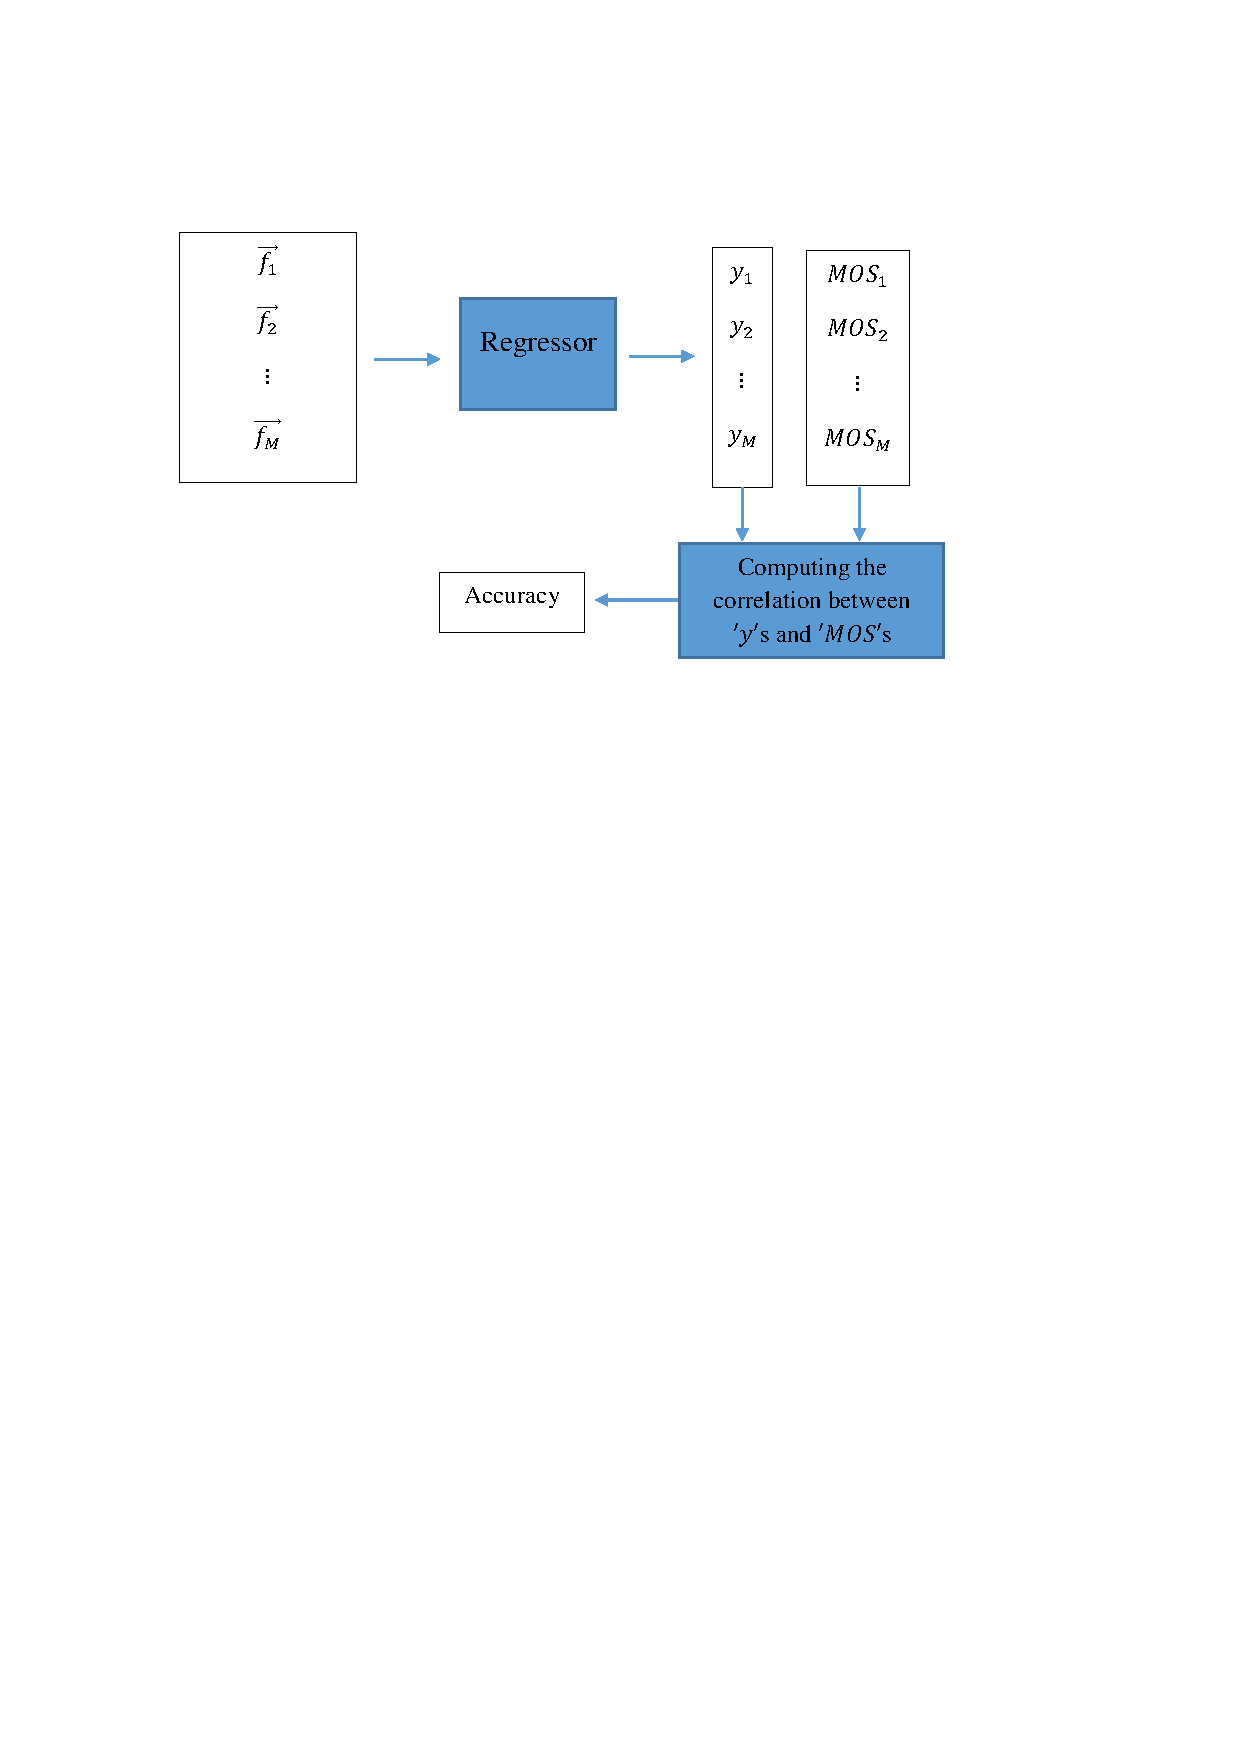
\includegraphics[width=0.97\textwidth, trim={2.8cm 18.3cm 4.8cm 3.8cm}, clip]{./figs/fg_svr_test}}
    \caption{Testing feature-based methods (The `Regressor' is the output of the train process.)}
    \label{fig:svr_test}
\end{figure}
If a dataset contains $N$ pictures and their corresponding human scores, it can be considered as a set of ordered pairs like $(I_i, MOS_i)$, where $I_i$ is the $i^{th}$ image and $MOS_i$ is the subjective score of $I_i$ for $i\in\{1,2,\ldots, N\}$. These ordered pairs are the `samples'. If a feature vector is extracted from $I_i$ it will be named: $\Vec{f}_i$. If $L$ samples of the dataset are selected for train, and, $M$ samples for test, a model can be trained on $L$ samples (Fig.~\ref{fig:svr_train}) and tested on the other $M$ samples (Fig.\ref{fig:svr_test}). It must be noted that $L+M=N$. The more the scores of the model are correlated with $MOS$s, the better is the performance of the method. The learning model in this framework can be a SVR~\cite{Vapnik1995} or a neural network. Although this model is effective in method's performance, but the main contribution to accuracy and speed, is made by the feature extraction mechanism.

Natural scene statistics is a common criterion for extracting features. Consider the two pictures in Fig.~\ref{fig:mscnhst} of `bikes' and `monarch' butterfly. If these images are transformed to MSCN\footnote{Calculation of the \emph{Mean-Subtracted \& Contrast-Normalized} image will be explained in the following paragraphs.} domain, their frequency histogram will obey the normal distribution (Fig.~\ref{fig:mscnhst_hst_bikes} and Fig.~\ref{fig:mscnhst_hst_monarch}). Ruderman~\cite{Ruderman1994} demonstrated that this distribution will be normal for any natural image, regardless of its content. If an image is distorted, it deviates from the natural state and it is expected that its distribution in the MSCN domain deviates from the normal distribution.
\begin{figure}
     \centering
     \begin{subfigure}[b]{0.3\textwidth}
         \centering
         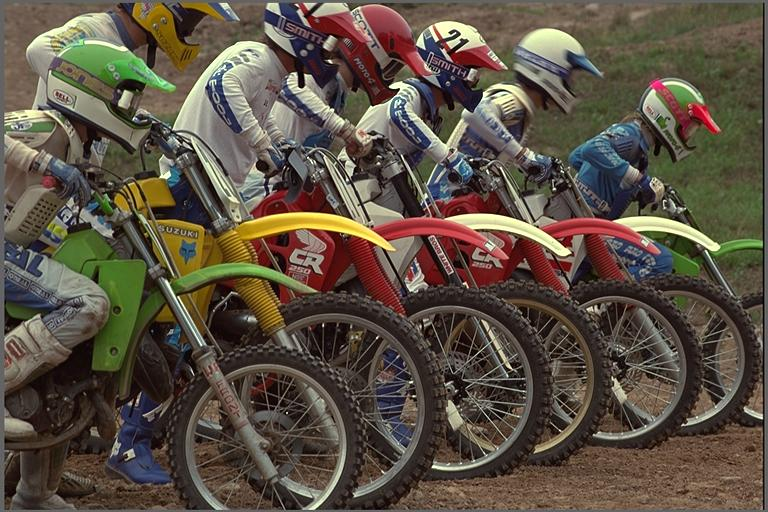
\includegraphics[width=\textwidth]{./figs/reference}
         \caption{`bikes'}
         \label{fig:mscnhst_bikes}
     \end{subfigure}
     \hfill
     \begin{subfigure}[b]{0.3\textwidth}
         \centering
         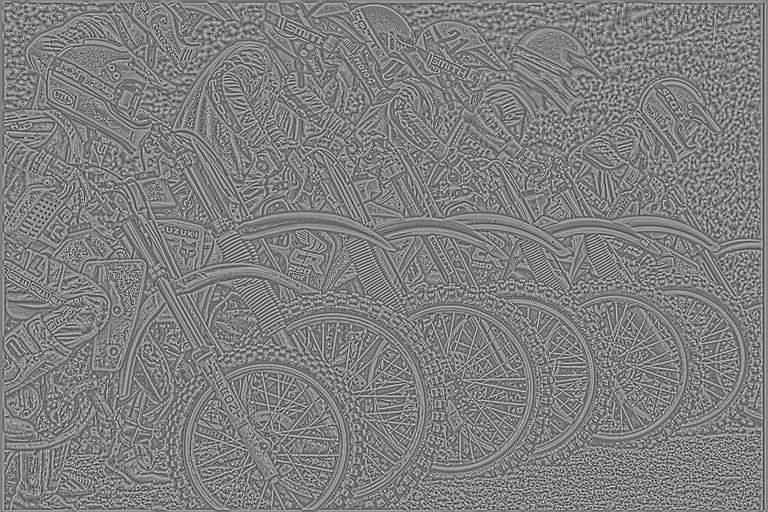
\includegraphics[width=\textwidth]{./figs/mscn_reference}
         \caption{MSCN version of `bikes'}
         \label{fig:mscnhst_mscn_bikes}
     \end{subfigure}
     \hfill
     \begin{subfigure}[b]{0.3\textwidth}
         \centering
         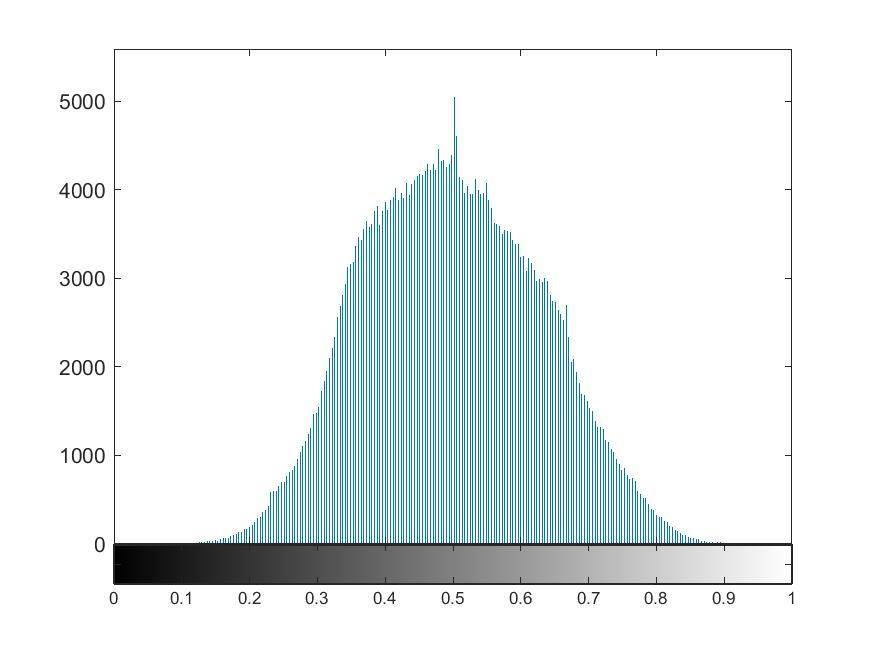
\includegraphics[width=\textwidth]{./figs/mscn_histreference}
         \caption{histogram of MSCN map}
         \label{fig:mscnhst_hst_bikes}
     \end{subfigure}
     \\
     \begin{subfigure}[b]{0.3\textwidth}
         \centering
         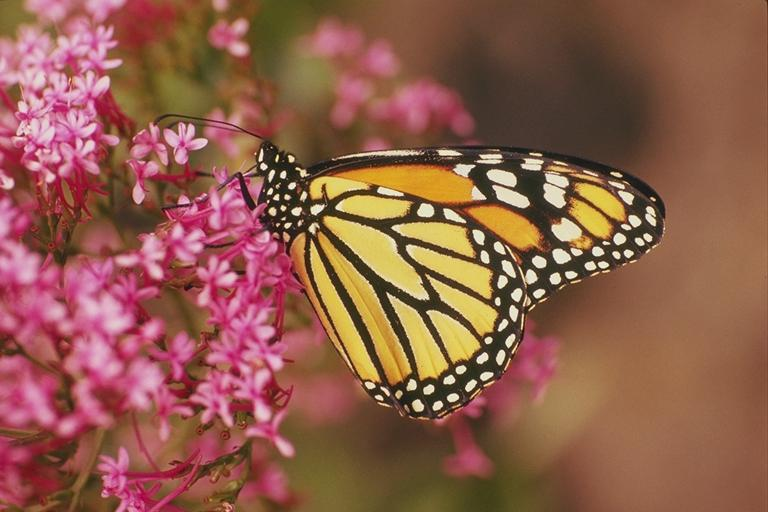
\includegraphics[width=\textwidth]{./figs/monarch}
         \caption{`monarch'}
         \label{fig:mscnhst_monarch}
     \end{subfigure}
     \hfill
     \begin{subfigure}[b]{0.3\textwidth}
         \centering
         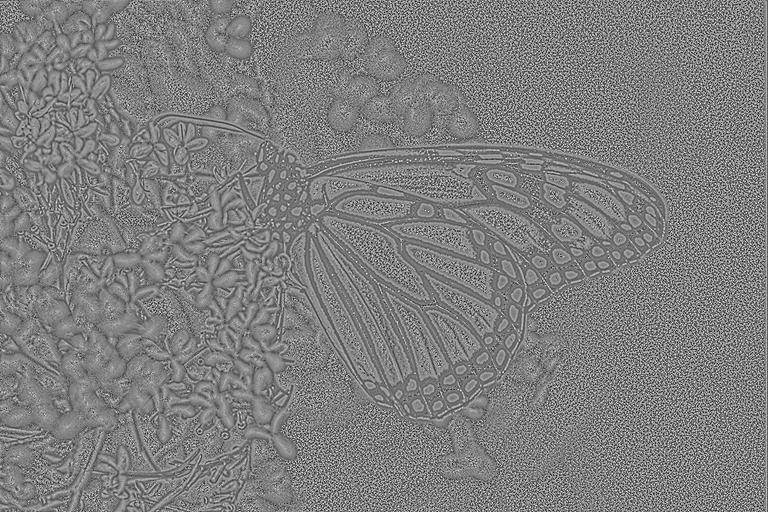
\includegraphics[width=\textwidth]{./figs/mscn_monarch}
         \caption{MSCN map of `monarch'}
         \label{fig:mscnhst_mscn_monarch}
     \end{subfigure}
     \hfill
     \begin{subfigure}[b]{0.3\textwidth}
         \centering
         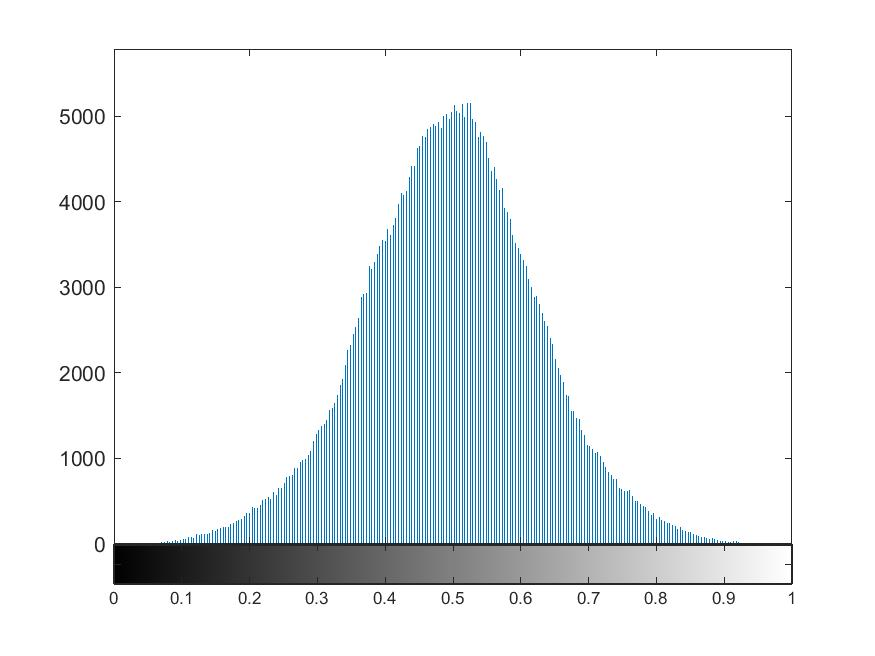
\includegraphics[width=\textwidth]{./figs/mscn_histmonarch}
         \caption{histogram of MSCN map}
         \label{fig:mscnhst_hst_monarch}
     \end{subfigure}
        \caption{Two images from LIVE dataset and their MSCN map and the histogram of values in the MSCN domain}
        \label{fig:mscnhst}
\end{figure}
In Fig~\ref{fig:nss} the histogram of MSCN maps are shown for the distorted versions of `bikes' and `monarch'. It is seen that despite the different contents of the two images, the distributions change with respect to type, and intensity of the distortions. For example, the Jpeg histogram has the same shape for both scenes (Fig.~\ref{fig:nss10} and Fi.g~\ref{fig:nss11}). Therefore, the MSCN distribution of a picture can be used to detect distortion.
\begin{figure}
     \centering
     \begin{subfigure}[b]{0.23\textwidth}
         \centering
         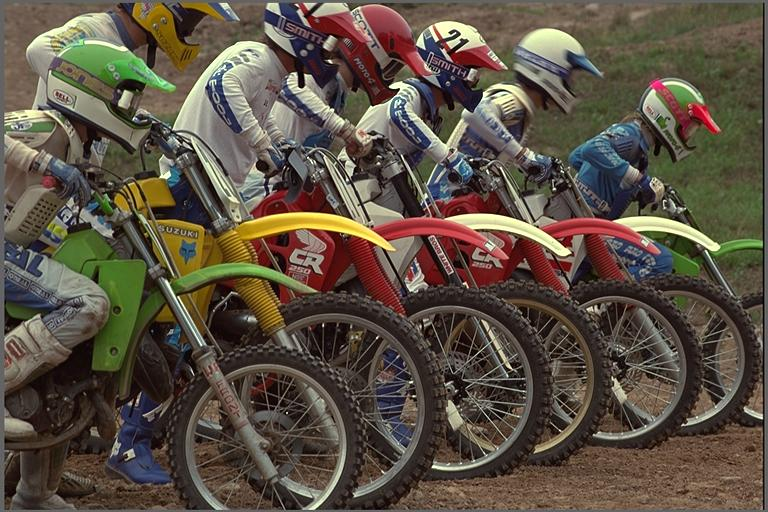
\includegraphics[width=\textwidth]{./figs/reference}
         \caption{}
         \label{fig:nss1}
     \end{subfigure}
     %\hfill
     \begin{subfigure}[b]{0.23\textwidth}
         \centering
         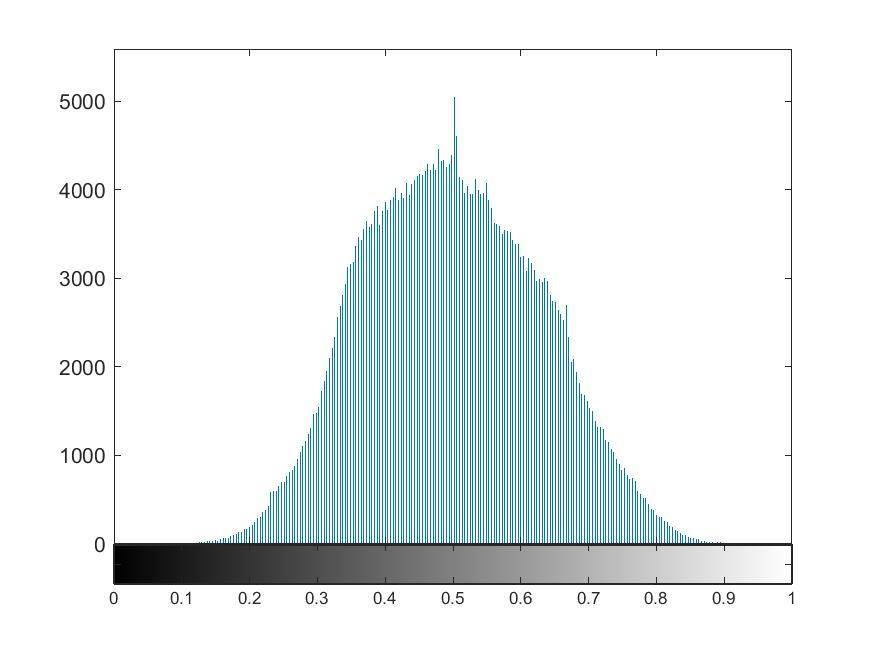
\includegraphics[width=\textwidth]{./figs/mscn_histreference}
         \caption{}
         \label{fig:nss2}
     \end{subfigure}
     %\hfill
     \begin{subfigure}[b]{0.23\textwidth}
         \centering
         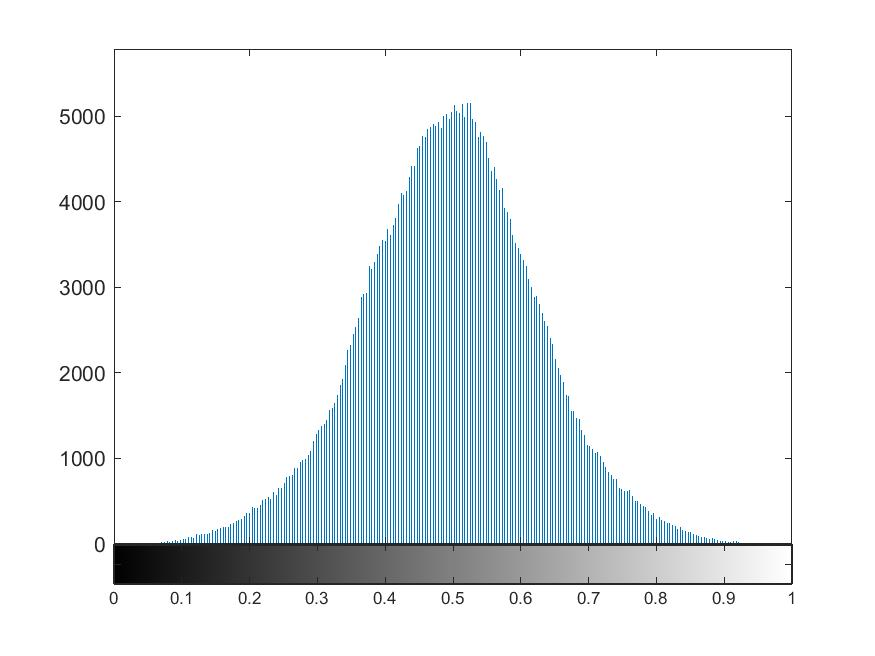
\includegraphics[width=\textwidth]{./figs/mscn_histmonarch}
         \caption{}
         \label{fig:nss3}
     \end{subfigure}
     \begin{subfigure}[b]{0.23\textwidth}
         \centering
         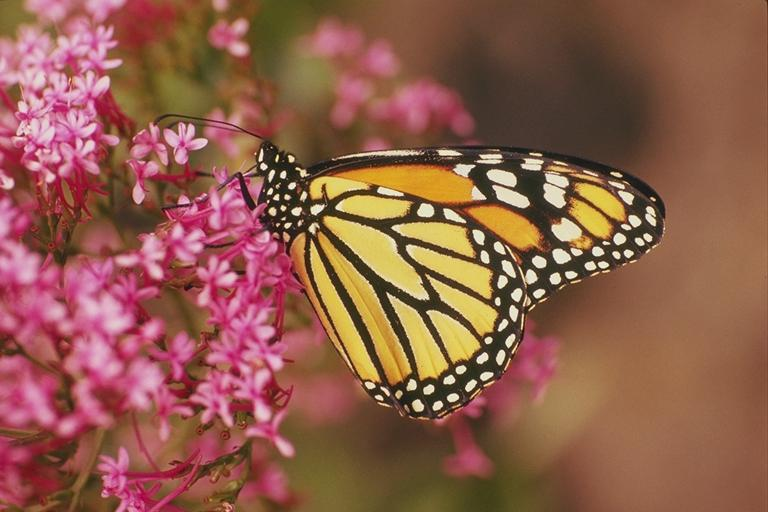
\includegraphics[width=\textwidth]{./figs/monarch}
         \caption{}
         \label{fig:nss4}
     \end{subfigure}
     \\
     \begin{subfigure}[b]{0.23\textwidth}
         \centering
         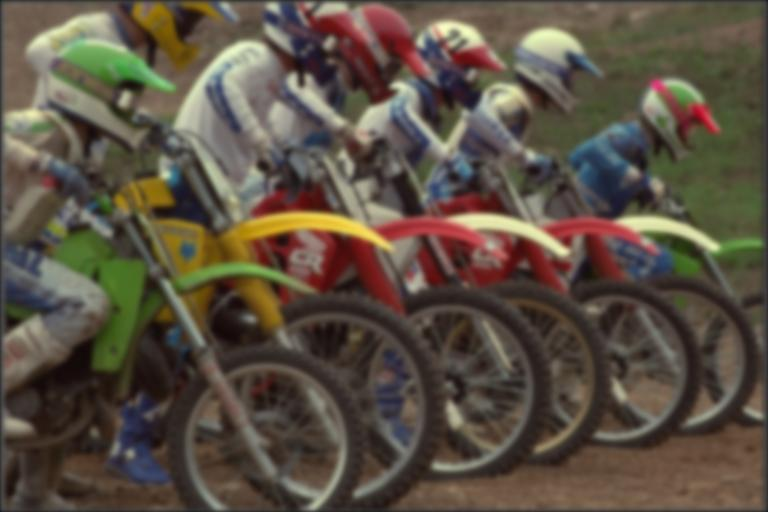
\includegraphics[width=\textwidth]{./figs/blur}
         \caption{}
         \label{fig:nss5}
     \end{subfigure}
     %\hfill
     \begin{subfigure}[b]{0.23\textwidth}
         \centering
         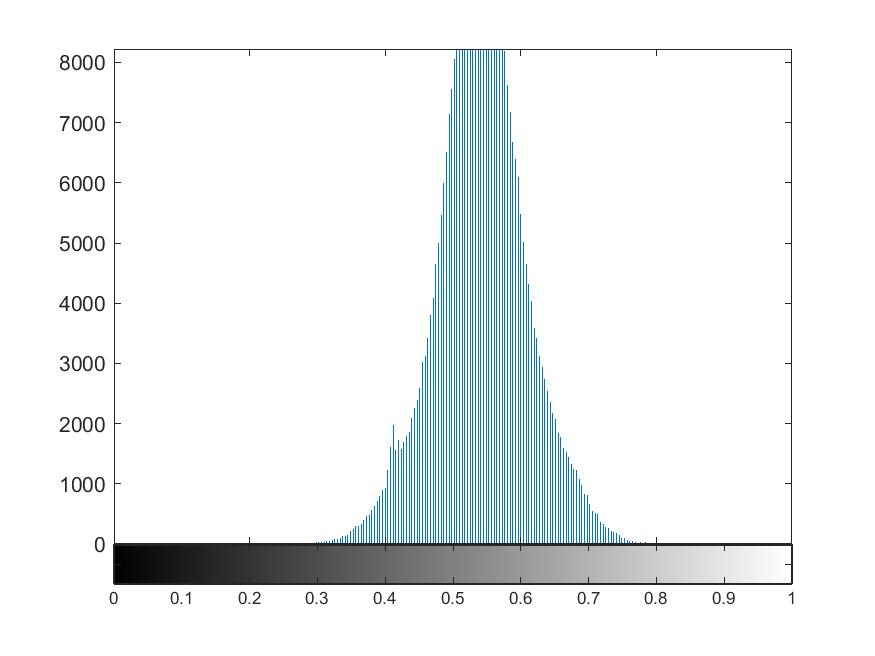
\includegraphics[width=\textwidth]{./figs/mscn_histblur}
         \caption{}
         \label{fig:nss6}
     \end{subfigure}
     %\hfill
     \begin{subfigure}[b]{0.23\textwidth}
         \centering
         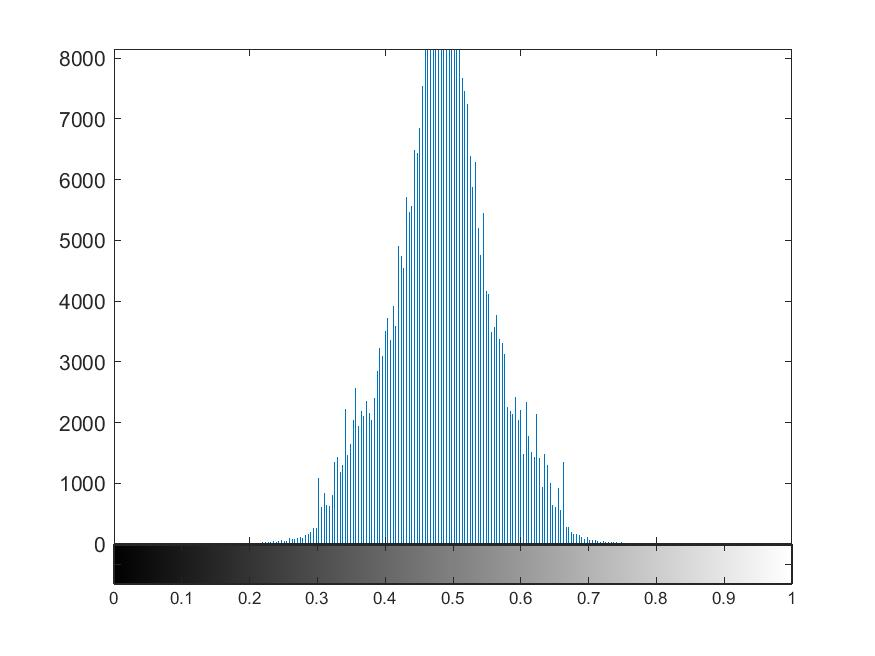
\includegraphics[width=\textwidth]{./figs/mscn_histmblur}
         \caption{}
         \label{fig:nss7}
     \end{subfigure}
     \begin{subfigure}[b]{0.23\textwidth}
         \centering
         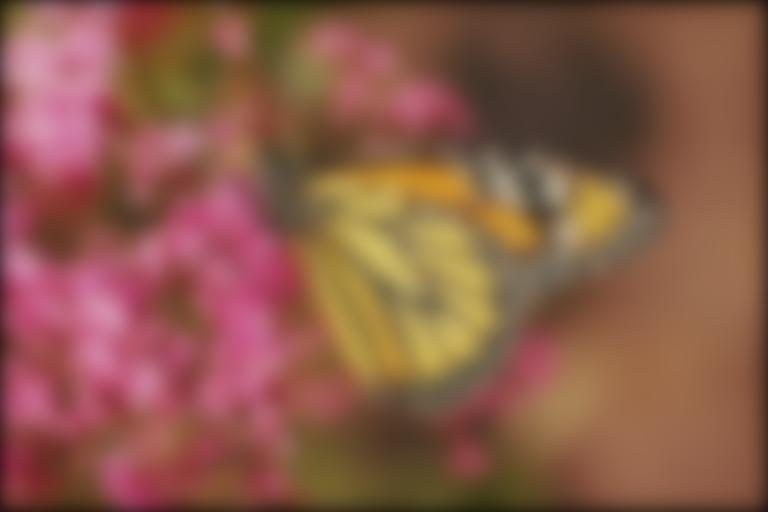
\includegraphics[width=\textwidth]{./figs/mblur}
         \caption{}
         \label{fig:nss8}
     \end{subfigure}
     \\
     \begin{subfigure}[b]{0.23\textwidth}
         \centering
         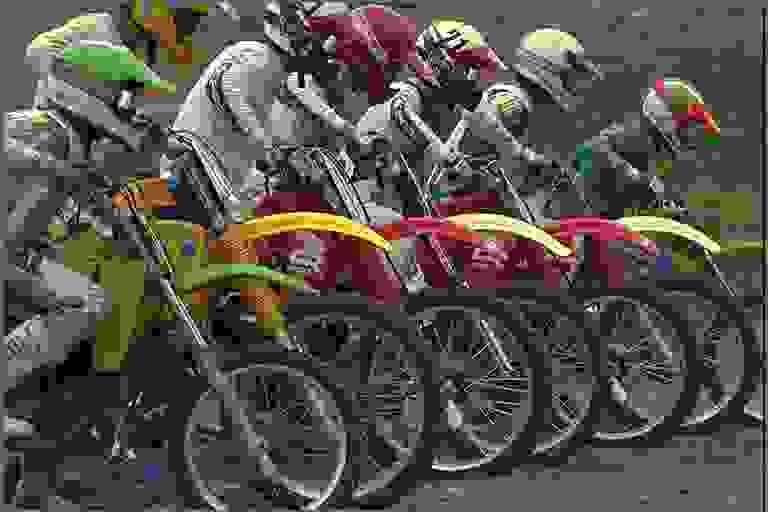
\includegraphics[width=\textwidth]{./figs/jpeg}
         \caption{}
         \label{fig:nss9}
     \end{subfigure}
     %\hfill
     \begin{subfigure}[b]{0.23\textwidth}
         \centering
         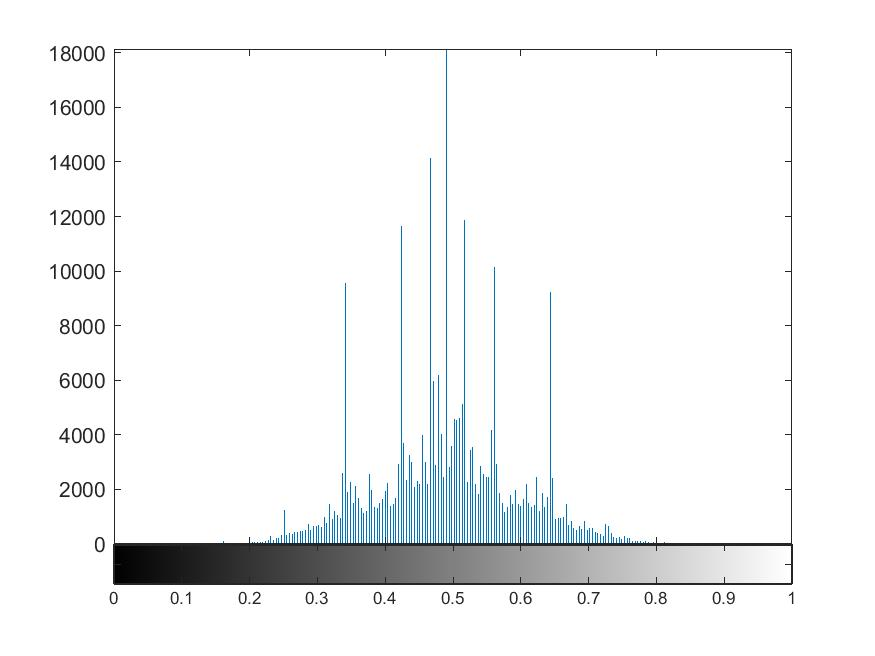
\includegraphics[width=\textwidth]{./figs/mscn_histjpeg}
         \caption{}
         \label{fig:nss10}
     \end{subfigure}
     %\hfill
     \begin{subfigure}[b]{0.23\textwidth}
         \centering
         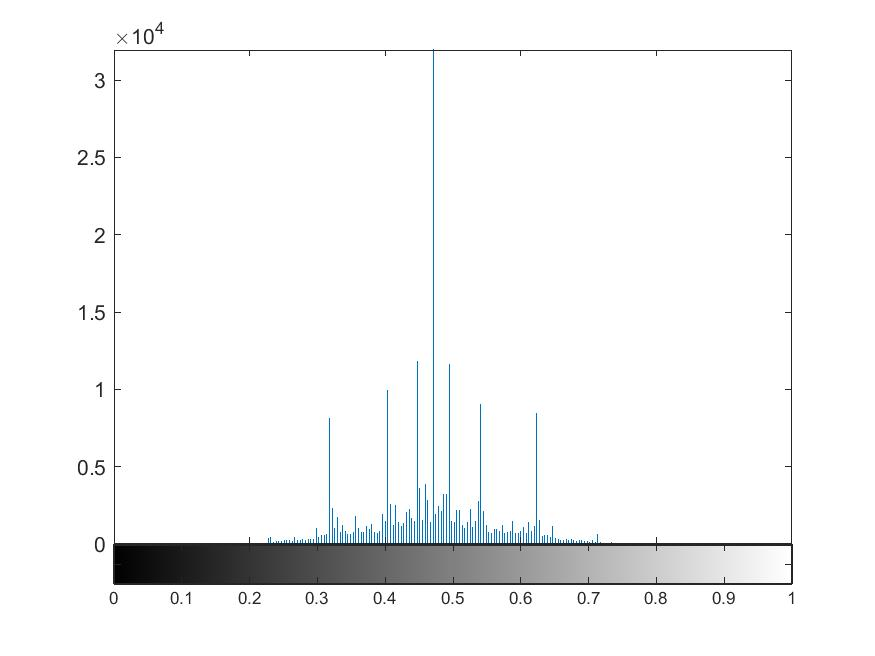
\includegraphics[width=\textwidth]{./figs/mscn_histmjpeg}
         \caption{}
         \label{fig:nss11}
     \end{subfigure}
     \begin{subfigure}[b]{0.23\textwidth}
         \centering
         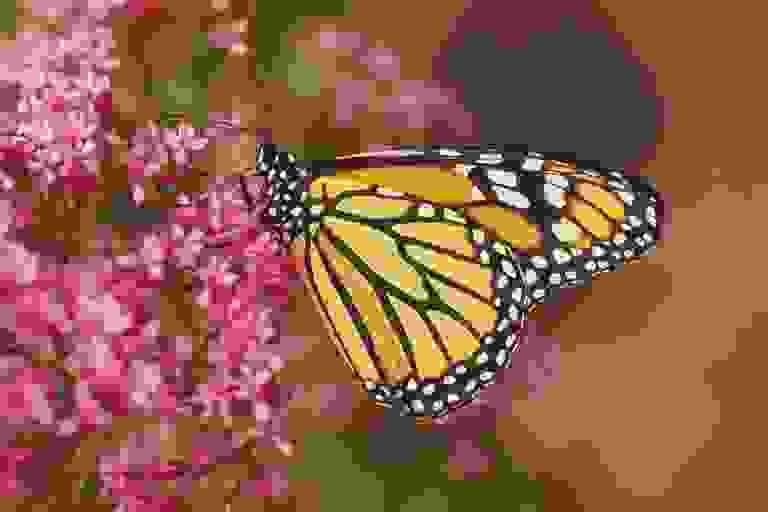
\includegraphics[width=\textwidth]{./figs/mjpeg}
         \caption{}
         \label{fig:nss12}
     \end{subfigure}
     \\
     \begin{subfigure}[b]{0.23\textwidth}
         \centering
         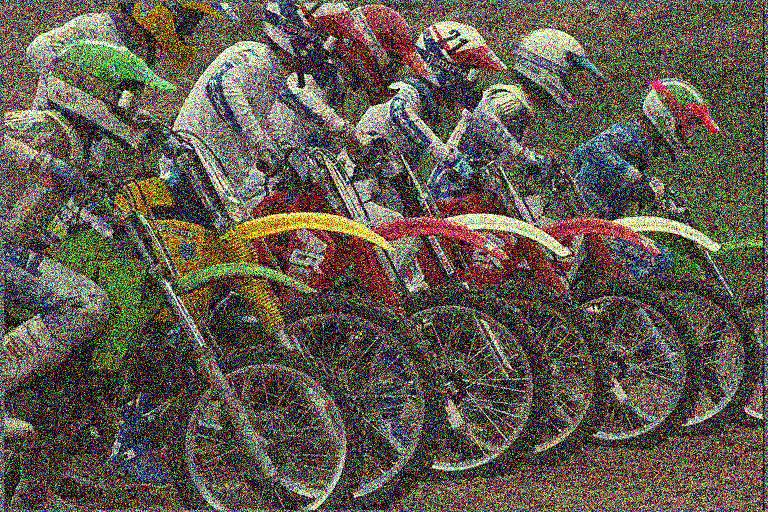
\includegraphics[width=\textwidth]{./figs/noise}
         \caption{}
         \label{fig:nss13}
     \end{subfigure}
     %\hfill
     \begin{subfigure}[b]{0.23\textwidth}
         \centering
         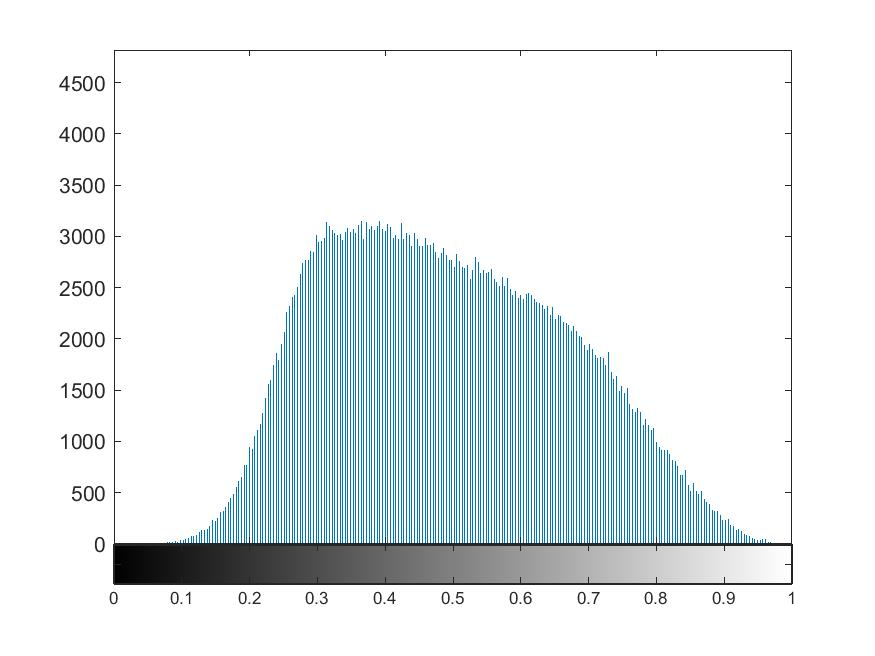
\includegraphics[width=\textwidth]{./figs/mscn_histnoise}
         \caption{}
         \label{fig:nss14}
     \end{subfigure}
     %\hfill
     \begin{subfigure}[b]{0.23\textwidth}
         \centering
         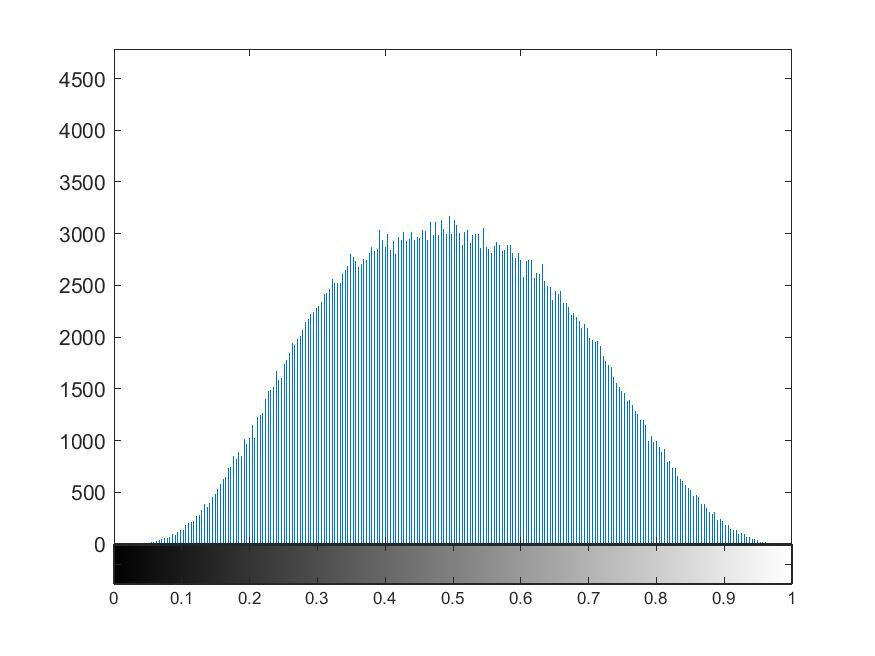
\includegraphics[width=\textwidth]{./figs/mscn_histmnoise}
         \caption{}
         \label{fig:nss15}
     \end{subfigure}
     \begin{subfigure}[b]{0.23\textwidth}
         \centering
         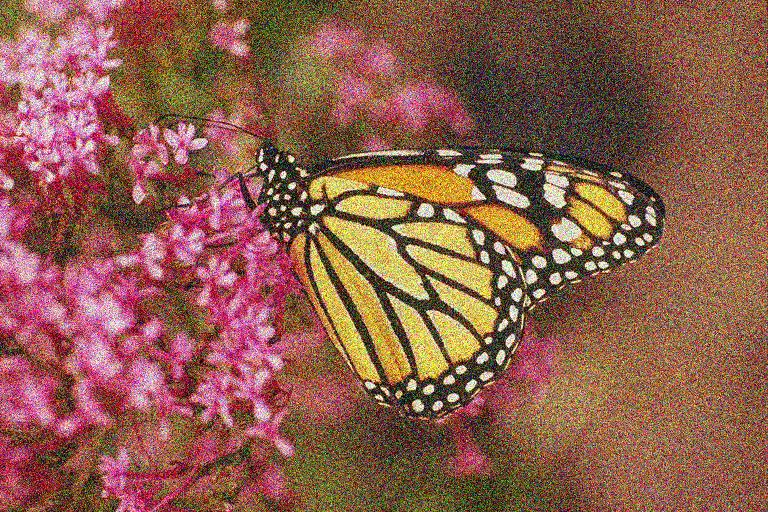
\includegraphics[width=\textwidth]{./figs/mnoise}
         \caption{}
         \label{fig:nss16}
     \end{subfigure}
        \caption{MSCN distributions for distorted versions of two images}
        \label{fig:nss}
\end{figure}
The MSCN value of the pixel at $(x, y)$ of the grayscale image $I$ is represented with $\hat{I}(x, y)$ and obtained from the following relation~\cite{Mittal2012a}:
\begin{equation}
    \hat{I}(x, y) = \frac{I(x, y)-\mu}{\sigma}
    \label{eq:mscn}
\end{equation}
Where $\mu$ and $\sigma$ are the mean and variance in a $3\times3$ neighborhood of $I(x, y)$. 

The distribution of MSCN values can also be fitted with a generalized Gaussian distribution (GGD)~\cite{sharifi1995estimation}. GGD has parameters, such as mean ($m$), variance ($\sigma$), and shape ($\alpha$). The estimated parameters for an image, can be considered as the elements of a feature vector that describes the quality of the image.

In fact, this is what the method BRISQUE~\cite{Mittal2012a} does. Beside MSCN coefficients, NSS of other domains have been explored. BIQI~\cite{Moorthy2010} uses NSS in wavelet domain and BLIINDS-II~\cite{Saad2012} computes the features based on the entropy and average of coefficients of discrete cosine transform (DCT). Also, other distributions have been used for describing the histograms such as Gaussian scale mixtures (GSM)~\cite{Gupta2018}.
%---------------------------------------------
\subsection{Automatic Feature Extraction}
%---------------------------------------------
Convolutional neural networks can also extract feature vectors~\cite{Badrinarayanan2017}. The common architecture of these networks pools multiple 2D-feature maps after many convolutional layers to a 1D-vector. Then, fully connected layers of neurons classify or regress the vector. Methods like CNN~\cite{Kang2014}, MEON~\cite{Ma2017a}, DIQaM-NR~\cite{Bosse2018}, and Rank-IQA~\cite{liu2017rankiqa} are examples of such networks.

Using CNNs, the feature extraction process is embedded in the network and it is difficult to interpret the computed features. This is the same for dictionary-based methods~\cite{Jurie2005}. In these methods, such as CORNIA~\cite{Ye2012b}, HOSA~\cite{Xu2016}, QAF~\cite{Zhang2014}, SOM~\cite{Zhang2015b}, and QAC~\cite{Xue2013}, the distorted image is coded in a feature vector, based on a dictionary that contains the features of all good images. This dictionary is built by clustering the features of a set of good quality images.

Automatic features are shown to be expressive. In neural networks, these features are jointly optimized with the model that computes the scores, which increases the accuracy. However, the computational complexity of these methods is high and they demand large numbers of training samples. As mentioned earlier, these features are not interpretable and their relation with quality aspects of the image cannot be analyzed.
% --------------------------------------------
\section{FR methods for Multiple Distortions}
% --------------------------------------------
The existence of multiple distortions in an image, makes quality prediction difficult~\cite{Chandler2013}. Even if we can measure the severity of each distortion correctly, their \emph{joint effect} on the perceived quality will be difficult to predict, since their combination is not linear and depends on the type of distortions~\cite{goodman1979multidimensional}. The accurate measurement of distortions' intensity in the presence of other distortions, is also controversial~\cite{linde1981similarity} and necessitates to consider the \emph{mutual effect} of the distortions on each other. As an example, assume adding a fixed amount of noise to two images; a sharp image and its blurry version. Normally the noise will be more sensible in the blurry version. Similarly, it is expected that blurring a noisy image must alleviate the effect of noise~\cite{linde1981similarity}. However, subjective experiments~\cite{Kayargadde1996} show that this is true in some cases and completely wrong for many common samples.

These observations show the difficulty of assessing multiple distortions and reveal that accurate prediction of each combination or even permutation of distortions can be quite different. Thus, optimization for a specific permutation may result in poor performance for others. Some of methods for multiple distortions, tried to estimate or model the joint and mutual effect of the distortions. In the rest of the section, different methods for IQA of multiply-distorted images are reviewed and analyzed.
% --------------------------------
\subsection{Combination of Scores}
% --------------------------------
Combining the scores of four singly-distorted metrics, was the solution for FR IQA of multiple distortions, proposed by Chetouani~\cite{Chetouani2016}. In this method, four scores are computed for the distorted image with methods VIF~\cite{Sheikh2006}, IFC~\cite{Sheikh2005}, WASH~\cite{Reenu2013}, and SSIM~\cite{Wang2004}. They are then fed to an SVR as a $1\times 4$ feature vector to be mapped to the quality score.

The four single distortion methods that are employed here, consider different criteria. SSIM measures structural similarity, VIF and IFC take images' entropy into account and WASH measures blurriness. With this combination, it has been tried to capture the effect of multiple distortions.

A similar approach was taken by Okarma in~\cite{Okarma2014} with the difference that a nonlinear combination of the scores was used to pool the scores of the single metrics to the final score. The coefficients and powers of this nonlinear combination were optimized using the subjective scores of multi-distortion IQA datasets.

Due to the difficulty of modeling the joint effect, Chetouani used SVR in order to let machine learning to estimate the correct combination based on the individual metrics. However, when using a trainable model, its ability to generalize to samples outside the training dataset must be tested as well. Meanwhile, FR methods are normally based on mathematical relation and compute the quality directly.

Another issue is that the methods in~\cite{Chetouani2016} and~\cite{Okarma2014} need to execute multiple independent metrics which is a huge computational load. This makes them very slow in comparison to the conventional FR metrics.
% -----------------------------------------------
\subsection{Similarity of QWT Subbands}
% ------------------------------------------------
Li et al.~\cite{Li2018a} used quaternion wavelet transform (QWT)~\cite{Muraleetharan2015} for extracting image structural information. At each scale, an image in QWT domain is decomposed into four subbands, $LL$, $LH$, $HL$, and $HH$. Each of these subbands has a magnitude, $M$, and three phases, $\theta$, $\phi$, and $\psi$ (Fig.~\ref{fig:qwt}).
\begin{figure}
     \centering
     \begin{subfigure}[b]{0.23\textwidth}
         \centering
         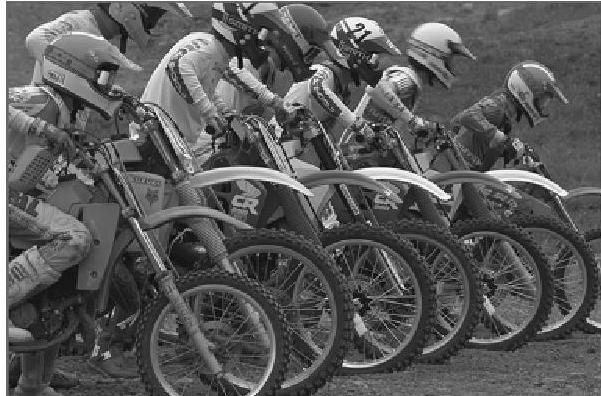
\includegraphics[width=\textwidth]{./figs/m_1_1_q}
         \caption{$LL_M$}
         \label{fig:qwt1}
     \end{subfigure}
     %\hfill
     \begin{subfigure}[b]{0.23\textwidth}
         \centering
         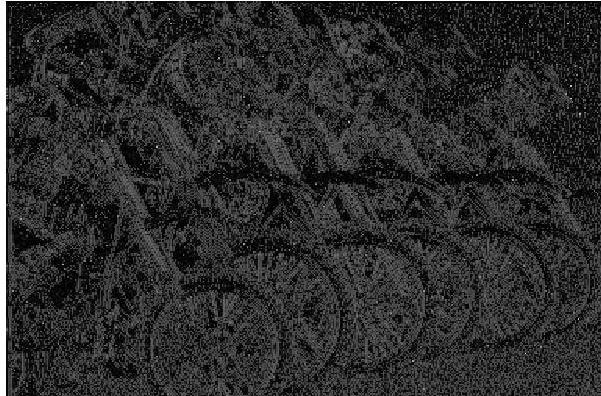
\includegraphics[width=\textwidth]{./figs/o_1_1_1_q}
         \caption{$LL_{\theta}$}
         \label{fig:qwt2}
     \end{subfigure}
     %\hfill
     \begin{subfigure}[b]{0.23\textwidth}
         \centering
         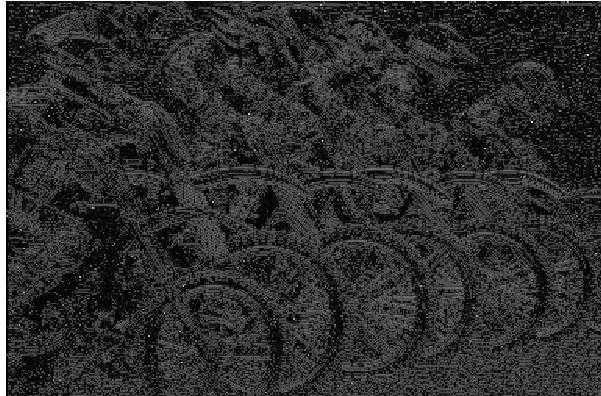
\includegraphics[width=\textwidth]{./figs/o_1_1_2_q}
         \caption{$LL_{\phi}$}
         \label{fig:qwt3}
     \end{subfigure}
     \begin{subfigure}[b]{0.23\textwidth}
         \centering
         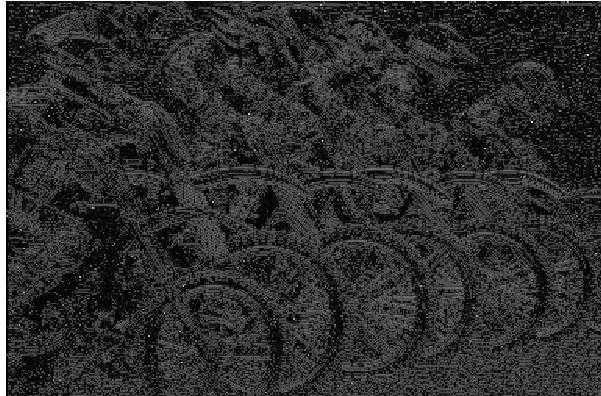
\includegraphics[width=\textwidth]{./figs/o_1_1_2_q}
         \caption{$LL_{\psi}$}
         \label{fig:qwt4}
     \end{subfigure}
     \\
     \begin{subfigure}[b]{0.23\textwidth}
         \centering
         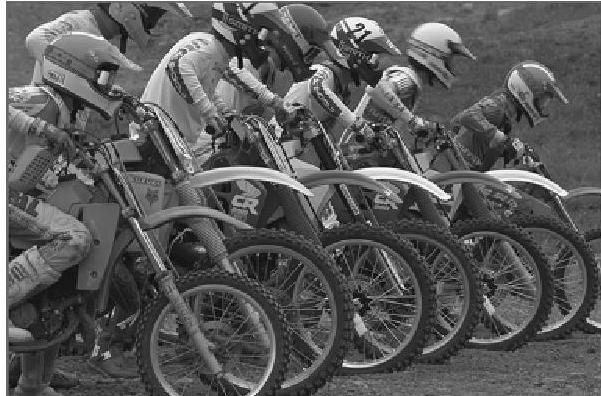
\includegraphics[width=\textwidth]{./figs/m_1_1_q}
         \caption{$LH_M$}
         \label{fig:qwt5}
     \end{subfigure}
     %\hfill
     \begin{subfigure}[b]{0.23\textwidth}
         \centering
         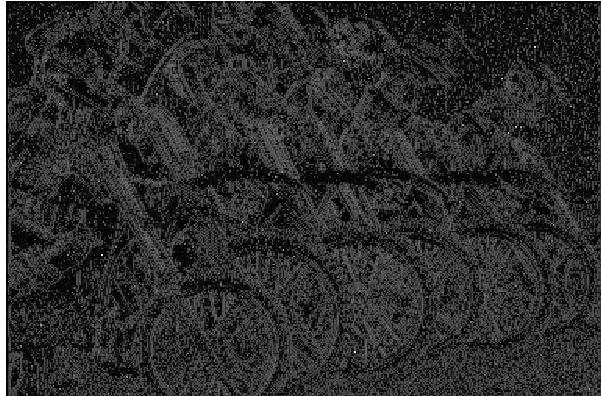
\includegraphics[width=\textwidth]{./figs/o_1_2_1_q}
         \caption{$LH_{\theta}$}
         \label{fig:qwt6}
     \end{subfigure}
     %\hfill
     \begin{subfigure}[b]{0.23\textwidth}
         \centering
         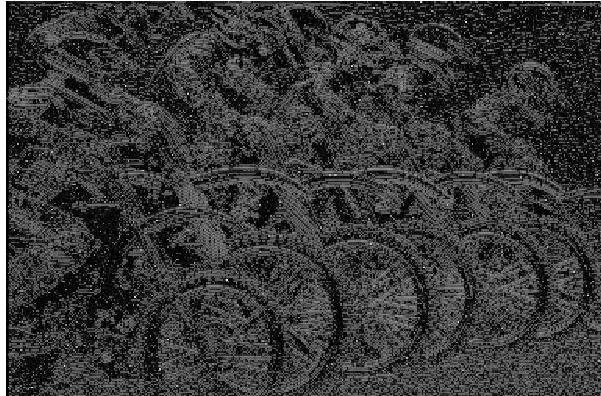
\includegraphics[width=\textwidth]{./figs/o_1_2_2_q}
         \caption{$LH_{\phi}$}
         \label{fig:qwt7}
     \end{subfigure}
     \begin{subfigure}[b]{0.23\textwidth}
         \centering
         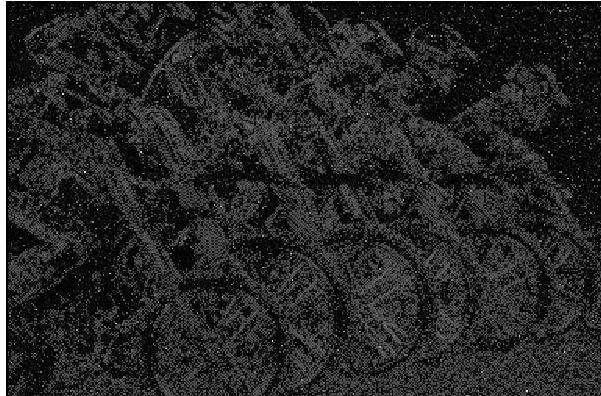
\includegraphics[width=\textwidth]{./figs/o_1_2_3_q}
         \caption{$LH_{\psi}$}
         \label{fig:qwt8}
     \end{subfigure}
     \\
     \begin{subfigure}[b]{0.23\textwidth}
         \centering
         \includegraphics[width=\textwidth]{./figs/m_2_1_q}
         \caption{$HL_M$}
         \label{fig:qwt9}
     \end{subfigure}
     %\hfill
     \begin{subfigure}[b]{0.23\textwidth}
         \centering
         \includegraphics[width=\textwidth]{./figs/o_2_1_1_q}
         \caption{$HL_{\theta}$}
         \label{fig:qwt10}
     \end{subfigure}
     %\hfill
     \begin{subfigure}[b]{0.23\textwidth}
         \centering
         \includegraphics[width=\textwidth]{./figs/o_2_1_2_q}
         \caption{$HL_{\phi}$}
         \label{fig:qwt11}
     \end{subfigure}
     \begin{subfigure}[b]{0.23\textwidth}
         \centering
         \includegraphics[width=\textwidth]{./figs/o_2_1_3_q}
         \caption{$HL_{\psi}$}
         \label{fig:qwt12}
     \end{subfigure}
     \\
     \begin{subfigure}[b]{0.23\textwidth}
         \centering
         \includegraphics[width=\textwidth]{./figs/m_2_2_q}
         \caption{$HH_M$}
         \label{fig:qwt13}
     \end{subfigure}
     %\hfill
     \begin{subfigure}[b]{0.23\textwidth}
         \centering
         \includegraphics[width=\textwidth]{./figs/o_2_2_1_q}
         \caption{$HH_{\theta}$}
         \label{fig:qwt14}
     \end{subfigure}
     %\hfill
     \begin{subfigure}[b]{0.23\textwidth}
         \centering
         \includegraphics[width=\textwidth]{./figs/o_2_2_2_q}
         \caption{$HH_{\phi}$}
         \label{fig:qwt15}
     \end{subfigure}
     \begin{subfigure}[b]{0.23\textwidth}
         \centering
         \includegraphics[width=\textwidth]{./figs/o_2_2_3_q}
         \caption{$HH_{\psi}$}
         \label{fig:qwt16}
     \end{subfigure}
        \caption{The QWT subbands of `bikes' in one scale}
        \label{fig:qwt}
\end{figure}
According to Fig.~\ref{fig:qwt}, subbands of QWT have fine characteristics for detecting distortions. The magnitude of $LL$, is an approximation of the entire image and roughly shift invariant. Phases of $LL$, demonstrate the horizontal, vertical and diagonal structures. The magnitudes of $LH$, $HL$, and $HH$, extract the edges in different directions. In their method, called QWT-IQA, Li et al. compare the magnitude and phases of subbands of the reference and distorted image. Then they compute the quality scores of each subband, which are named: $Q_{LL}$, $Q_{LH}$, $Q_{HL}$, and $Q_{HH}$.

The magnitude and phases are denoted as in Fig.~\ref{fig:qwt} and the corresponding terms in reference or distorted image, are distinguished with $R$ and $D$ subscripts. As an example, the computation of $Q_{LL}$ will be explained. To compare $LL_{M_R}$ and $LL_{M_D}$, their point-wise similarity will be calculated:
\begin{equation}
    LL_MS(x, y) = sim(LL_{M_D}(x, y), LL_{M_R}(x, y), c)
    \label{eq:LL_MS}
\end{equation}
$LL_MS$ is the similarity map of $LL_{M_D}$ and $LL_{M_R}$. Similarly, $LL_\theta S$, $LL_\phi S$, and $LL_\psi S$ can be calculated. To collapse the information in $LL_MS$, $LL_\theta S$, $LL_\phi S$, and $LL_\psi S$ into one map, their point-wise multiplication is calculated:
\begin{equation}
    LLS(x, y) = LL_MS^{10}(x, y)\times LL_\theta S(x, y)\times LL_\phi S(x, y)\times LL_\psi S(x, y)
    \label{eq:LLS}
\end{equation}
$LLS$ is the similarity map for the $LL$ subband of the reference and the distorted image. The power of $10$ for $LL_MS$ and $1$ for $LL_\theta S$, $LL_\phi S$, and $LL_\psi S$, is obtained experimentally. For pooling $LLS$ to one score, a weighted average of its values is computed. The weight of each pixel, $W(x, y)$, is the maximum of $LL_{M_R}$ and $LL_{M_D}$:
\begin{equation}
    W(x, y) = max\{LL_{M_R}(x, y), LL_{M_D}(x, y)\}
    \label{eq:weight_qwt}
\end{equation}
This weighting strategy is an effort to simulate an HVS property that relates to higher vision accuracy in brighter scenes~\cite{Gonzalez2008}. Pixels with larger values, correspond to brighter spots and contribute more in determining the quality score. The score of $LL$ is called $Q_{LL}$ and obtained from relation~\ref{eq:qwtiqa_LL}. The scores for other subbands can be computed similarly.
\begin{equation}
    Q_{LL} = \frac{\sum_x\sum_yLLS(x, y)\times W(x, y)}{\sum_x \sum_y W(x, y)}
    \label{eq:qwtiqa_LL}
\end{equation}
According to~\ref{eq:qwtiqa}, the final score is the linear combination of subbands' score. The values of coefficients $a$, $b$, $c$, and $d$ were optimized on MLIVE~\cite{Jayaraman2012} dataset.
\begin{equation}
    Q = a\times Q_{LL}+b\times Q_{LH}+c\times Q_{HL}+d\times Q_{HH}
    \label{eq:qwtiqa}
\end{equation}
QWT has been used for single-distortion assessments~\cite{chen2013image, traore2014reduced, Tang2017}. This transform is used in QWT-IQA for multiple distortions, however its time complexity is not suitable for real-time applications.
%-----------------------------------
\subsection{Measuring Mutual Information}
% -------------------------------------
IFC~\cite{Sheikh2005} is a FR method for single distortions which is defined based on the mutual information between the reference and the distorted image. IFC assumes that the distorted image is always a noisy and blurry version of the reference. The severity of noise and blur is estimated via NSS. This way, IFC measures the amount of information that can be extracted from the reference, but not from the distorted image. VIF~\cite{Sheikh2006} is the improved version of this algorithm.

In MDIQA~\cite{zhang2019full}, IFC is modified for multiple distortions. IFC extracts NSS from the reference and the distorted in wavelet domain. Due to its model of distortion, IFC considers the mutual effect. In MDIQA, the wavlet subbands are filtered with contrast sensitivity function~\cite{ngan1986cosine}, prior to NSS extraction.

The implementations that authors provided for IFC are complex and MDIQA inherits the same complexity, yet with a minor increase in accuracy for multiple distortions.
% --------------------------------------------
\section{RR Methods for Multiple Distortions}
% --------------------------------------------
The methods presented so for, assumed that the reference image is one of the inputs to the algorithms. In the RR case, instead of the entire image, a feature vector of the image is available along with the distorted signal. The same features will be extracted from the distorted version and will be compared with the features of the reference. Similar to the FR scenario, the RR methods have been proposed specifically for multiply-distorted images and they will be reviewed in this section.
% ---------------------------------
\subsection{Combining Scores}
% ---------------------------------
Similar to~\cite{Chetouani2016}, a method was proposed in~\cite{Chetouani2015} to combine the features of distortion-specific measures for constructing the feature vector of the reference and the test images. NR methods for measuring the severity of blur, ringing effect, blocking effect, and noise extract features from the reference image and build the reference feature vector. The same algorithms are applied to the distorted image and build the distorted feature vector. The concatenation of these two vectors is fed to an SVR for quality prediction.

The SVR will estimate the mutual and joint effect of the measured distortions, however, like the FR case, the execution of multiple methods is computationally expensive.
% -------------------------------------------------
\subsection{Using the Internal Generative Mechanism}
% --------------------------------------------------
Mahmoudpour and Schelkens used the internal generative model~\cite{Friston2010} for assessing multiple
distortions~\cite{Mahmoudpour2017}. In this model, the image is decomposed to two subbands; the \emph{predicted} and the \emph{residual}. These two subbands are invariant to specific artifacts. The predicted image is variant to structural degradations, such as blur, but invariant to noise. On the other hand, the residual image is variant to noise, but is not sensitive to blur.

The predicted image is transformed to Shearlet domain to extract the edges of the image. The residual subband is described with Renyi entropy~\cite{Gabarda2007}. The final feature vector is obtained by subtracting the distorted vector from the reference vector and mapped to the score using SVR. This algorithm is improved in RRSEA~\cite{Mahmoudpour2018}. 
% ------------------------------------------
\section{NR methods for Multiple Distortions}
% ------------------------------------------
There has been more studies for the NR assessment of multiply-distorted images comparing to the FR and RR problems. In this section the methods are introduced with a review on their pros and cons.
% -----------------------------------------
\subsection{Five-Steps and Six-Steps Methods}
% ------------------------------------------
The first method proposed for NR assessment of multiply-distorted images was based on independent measurement of each distortion and the combining the measures into a single score for the entire image~\cite{Gu2013}. In the method called ``FISBLIM", Gu et al. mentioned that when HVS is exposed to a multiply-distorted scene, it primarily notes the noise of the image~\cite{Gonzalez2008}. There are mechanisms in the HVS that make the noise insensible~\cite{Dabov2007} and then eye notices other distortions.

In the first step, they estimate the noise severity with SINE~\cite{Zoran2009} and denoise the image based on the estimated intensity. Then they measure the blur and blocking effect of the noiseless image. The linear combination of these assessments gives the final score. In this framework, the severity of noise, blur and blocking effect can be measured with any distortion-specific method. Free energy principle~\cite{Friston2010} was incorporated in SISBLIM~\cite{Gu2014} to model human perception of distortion joint effect.

Although FISBLIM and SISBLIM are NR methods, they are not based on machine learning and compute the scores directly and could outperform conventional methods in assessing multiple distortions. These methods assume that the distortions of an image are a subset of noise, blur and Jpeg blocking artifact. This presumption limits their applications to images outside this set.
% ---------------------------------
\subsection{Combining Quality Parameters}
% ------------------------------------
It was shown in~\cite{Li2015relevant} that relevant perceptual features can describe the quality of images instead of measuring the distortions. Mean pixel value, image contrast, mean value of gradient magnitude, and a measure of texture complexity were the elements of the feature vector. Feature extraction is done in the spatial domain and the phase congruency of Fourier domain. In LQAF-RF~\cite{Ma2017forest} a random forest replaced SVR for mapping the features to quality in order to estimate the joint effect of the distortions. In~\cite{Li2018access} authors analysed the image in multiple scales which improved the accuracy, but caused a slower execution.
% --------------------------------------------------
\subsection{Dictionary-Based Approach}
% --------------------------------------------------
BRISQUE~\cite{Mittal2012a}, BIQI~\cite{Moorthy2010}, and SRNSS~\cite{He2012srnss} are NR methods for singly-distorted images, that each of them extracts 36, 18, and 24 features out of an image, respectively. If we apply all of them to an image, we will have 87 features. Authors in BoWSF~\cite{lu2015no} measured the correlation of each of these 87 features with the severity of specific distortions in presence of other distortions. More correlated features were assumed to be more robust to the mutual effect of the distortions. So they ended up with a subset of features, called the `selected features'.

If we consider a set of $N$ good-quality images, we can clip $P$ patches from each of them and obtain $N\times P$ good-quality patches (Fig.~\ref{fig:dic}). By extracting the selected features from good-quality patches, we have $N\times P$ vectors. $K$-means clustering of these vectors will result in $K$ vectors that are the center of each cluster. These $K$ center-vectors will serve as the dictionary that describes a good quality image. For a test image, $P$ patches are extracted and described by the selected features in BoWSF. The Euclidean distance of these vectors with the $K$ centers, composes the feature vector that describes the entire image. Lasso regression~\cite{Tibshirani1996} is then used to map the vector to score.
\begin{figure}
    \centering
    \fbox{\includegraphics[width=0.97\textwidth, trim={3cm 13.8cm 3.5cm 3.3cm}, clip]{./figs/fg_dic}}
    \caption{The procedure of building a dictionary}
    \label{fig:dic}
\end{figure}

It was shown in~\cite{Legge1980} that different distortions appear differently in smooth or detailed image regions. For example, noise is less perceivable in crowded image regions. Clipping patches from various areas of an image, gives BoWSF the chance to consider the effect of distortion on different regions of image.
% -----------------------------------------------------
\subsection{Learning to Measure Distortion Combinations}
% -----------------------------------------------------
Zhang and Chandler~\cite{Zhang2018} artificially distorted the images of Berkeley dataset~\cite{Martin2001} to create a set of multiply distorted images. Each image in their synthesized dataset falls into one of these seven categories:
\begin{itemize}
    \item Only blurred
    \item Only noisy
    \item Only compressed with Jpeg algorithm
    \item Blurred and noised
    \item Blurred and compressed
    \item Compressed and noisy
    \item Compressed, noisy, and blurred
\end{itemize}
The images of each category vary in severity of the distortions. Like BoWSF~\cite{lu2015no}, they measured the correlation of different features with different distortion levels. They experimented the features of GWH-GLBP~\cite{Li2016}, C-DIIVINE~\cite{Zhang2014cdiivine}, and DESIQUE~\cite{Zhang2013desique}, then chose the most correlated ones as the `selected features'. 

A classifier was trained to categorize an image into one of the seven mentioned classes based on the selected features. For each class, three SVRs were trained to measure the severity of blur, noise, and compression loss.

Fig.~\ref{fig:dist_pam} illustrates the framework of this method, named `MUSIQUE'. The classifier uses the selected features to output seven probabilities, $P(i)$s, where $i\in\{1,2,\ldots, 7\}$ and $\sum_{i=1}^{7}P(i)=1$. $P(i)$ is the probability that the image belongs to $i^{th}$ distortion category. The selected features are also fed to seven groups of SVRs. In the group $i$, three SVRs are trained: one for estimating $B_i$ (level of blur), one for $N_i$ (level of noise), and one for $J_i$ (level of Jpeg compression). That is for each $\mathscr{D}_i$ , where $\mathscr{D}\in \{B, N, J\}$ and $i\in \{1,2,\ldots, 7\}$ a SVR is trained using the labeled distorted images. The final distortion parameters, $B$, $N$, and $J$, are obtained by the weighted average of $\mathscr{D}_i$s and $P(i)$s:
\begin{equation}
    N = \sum_{i=1}^7P(i)\times N_i
\end{equation}
\begin{equation}
    B = \sum_{i=1}^7P(i)\times B_i
\end{equation}
\begin{equation}
    J = \sum_{i=1}^7P(i)\times J_i
\end{equation}
The same pooling strategy in~\cite{Chandler2010} maps the three parameters to a quality score.

Although these models were trained merely on the synthesized database, they can be generalized to existing multiple-distortion datasets with acceptable accuracy. However, similar to FISBLIM, MUSIQUE is designed for particular distortions and is also a complicated and complex method. If we want to train MUSIQUE for four different distortions, the number of classes will increase from 7 to 15. 
\begin{figure}
    \centering
    \fbox{\includegraphics[width=0.97\textwidth, trim={4.4cm 13.8cm 2.7cm 4.2cm}, clip]{./figs/fg_dist_param}}
    \caption{Learning the distortion parameters}
    \label{fig:dist_pam}
\end{figure}
% ------------------------------------------
\subsection{Convolutional Neural Networks}
% ------------------------------------------
Kang et al.~\cite{Kang2014} proposed a deep architecture for IQA. The test image is transformed to MSCN domain and then divided to $32\times32$ patches. Each patch is mapped to a score by the network and the total score is the average of the patches. The images and scores in the subjective datasets are used for training the network. The architecture is shown in Fig.~\ref{fig:lekang}.
\begin{figure}
    \centering
    \fbox{\includegraphics[width=0.97\textwidth]{./figs/fig_lekang}}
    \caption{The architecture of Kang's network}
    \label{fig:lekang}
\end{figure}

The result of convolving a $32\times 32$ image with a $7\times 7$ filter with $stride=1$, is a $26\times 26$ feature map. By filtering the input patch with 50 filters, we will have 50 feature maps of dimension $26\times 26$. The maximum of each map is stored in a $1\times 50$ vector (max-pooling). The minimum of the maps is stored an another $1\times 50$ vector (min-pooling). All the elements of these two vectors are connected to the 800 neurons of the next layer. The output of these neurons is also connected to all of the 800 neurons in the next layer. The linear combination of these 800 outputs, is the final quality score. 

It can be inferred, that the two pooled vectors are the extracted features for the patch and the last fully-connected layers do the regression. Fu et al.~\cite{Fu2016} increased the number of filters from 50 to 400. They also used average-pooling, instead of max and min-pooling to collapse the feature maps. The resulted architecture was trained and tested on a subject-rated multiple distortion dataset. The modified network was more accurate for multiply-distorted images. 

EONSS~\cite{wang2019blind} is another CNN, proposed for multiple distortions. Different from previous networks, EONSS is not trained with subject-rated images. Deep neural networks need numerous training samples, hence the authors, trained EONSS on artificially distorted images that their scores were obtained from full-reference methods. This way they were not limited in the number of training samples, since both images and labels were synthesized. However, they tested the method on subjective datasets. Despite of being blind to human opinions (being `opinion-free'), the network could outperform other methods in terms of accuracy, but not speed. The architecture of EONSS is plotted in Fig.~\ref{fig:eonss}.
\begin{figure}
    \centering
    \fbox{\includegraphics[width=0.97\textwidth]{./figs/fig_eonss}}
    \caption{The architecture of EONSS}
    \label{fig:eonss}
\end{figure}
% --------------------------------------
\subsection{Using Local Binary Patterns}
% --------------------------------------
The method GWH-GLBP~\cite{Li2016} employed local binary patters (LBPs) to describe multiple distortions. LBP is an expressive descriptor in texture recognition~\cite{Ojala2002}. Consider 8 adjacent pixels of a center pixel. The value of the center pixel is either less or greater than the value of each neighbor. If a bit is assigned to this situation, an 8-bit binary number describes the value of the center pixel relative to its neighbors. The decimal equivalent of this binary number, will represent the center pixel in the LBP map. An image and its LBP map are demonstrated in Fig.~\ref{fig:lbp_orig}-\ref{fig:lbp_8,1}.
\begin{figure}
     \centering
     \begin{subfigure}[b]{0.3\textwidth}
         \centering
         \includegraphics[width=\textwidth]{./figs/gry_org009}
         \caption{original image}
         \label{fig:lbp_orig}
     \end{subfigure}
     \hfill
     \begin{subfigure}[b]{0.3\textwidth}
         \centering
         \includegraphics[width=\textwidth]{./figs/lbp_org009}
         \caption{$LBP_{8,1}$}
         \label{fig:lbp_8,1}
     \end{subfigure}
     \hfill
     \begin{subfigure}[b]{0.3\textwidth}
         \centering
         \includegraphics[width=\textwidth]{./figs/lbpRIU2_org009}
         \caption{$LBP_{8,1}^{riu2}$}
         \label{fig:lbpriu2sample}
     \end{subfigure}
        \caption{An image from MDID13 dataset along with its LBP map variants}
        \label{fig:im&Lbp}
\end{figure}

In the above explanations, 8 neighbors were considered that located at the radius 1 of the center pixel. If $P$ is the number of neighbors and $R$ is the radius, the LBP of pixel $I(x, y)$, can be formulated as:
\begin{equation}
    LBP_{P,R}(x, y) = \sum_{p=0}^{P-1}f\left(I\left(x+R cos\left(\frac{2 p  \pi}{P}\right),y+R sin\left(\frac{2 p  \pi}{P}\right)\right), I(x, y)\right).2^p
    \label{eq:lbp_P,R}
\end{equation}
Where $f$ outputs either $1$ or $0$ based on this definition:
\begin{equation}
%\[
    f(\alpha, \beta) = 
    \begin{cases}
        0 & \alpha-\beta < 0\\
        1 & \alpha-\beta \geq 0\\
    \end{cases}
%\]
\label{eq:f}
\end{equation}
It is apparent that $LBP_{8, 1}(x, y)$ can posses one of the $2^8=256$ possible values, but before converting it to a decimal number, we can count the number of transitions from $0$ to $1$ or from $1$ to $0$. If we categorize the binary patterns with respect to the number of their transitions, the class number of each pattern will be invariant to rotation. All binary patterns in Fig.~\ref{fig:roi} (figure form~\cite{Ojala2002}) have either two or zero transitions. It is shown in~\cite{Ojala2002} that these nine patterns have the best performance for describing images, which are invariant to rotation and luminance changes.
\begin{figure}
    \centering
    \fbox{\includegraphics[width = 0.98\textwidth]{figs/roi.jpg}}
    \caption{The nine possible binary patterns with 2 or less transitions}
    \label{fig:roi}
\end{figure}
The invariant LBP is called $LBP_{P, R}^{riu2}$ and formulated as:
\begin{equation}
    \begin{aligned}
        \lefteqn{LBP_{P, R}^{riu2}(x, y) =  }\\
        & & \begin{cases}
            \sum_{p=0}^{P-1}f\left( I\left(x+R cos\left(\frac{2 p  \pi}{P}\right),y+R sin\left(\frac{2 p  \pi}{P}\right)\right), I(x, y)\right) & \mathcal{U}\left(LBP_{P, R}(x, y)\right)\leq 2\\
            P+1 & o.w.
        \end{cases}
    \end{aligned}
    \label{eq:riu2}
\end{equation}
Where $I(x, y)$ and $f(., .)$ are the same as~\ref{eq:lbp_P,R} and~\ref{eq:f}; and $\mathcal{U}\left(LBP_{P, R}(x, y)\right)$ counts the transitions of the binary pattern of $LBP_{P, R}(x, y)$. The $LBP_{P, R}^{riu2}$, for $P=8$, can have 10 distinct values. Fig.~\ref{fig:lbpriu2sample} shows an example. 

It was shown in GHW-GLBP, that the LBP in gradient domain is effective in describing distortions. In this method, the gradient magnitude of the image is first computed and then described with an $LBP_{8, 1}^{riu2}$ operator. Fig.~\ref{fig:lbp_dsts} shows distorted versions of a scene along with their gradient magnitude and $LBP_{8, 1}^{riu2}$ maps.
\begin{figure}
     \centering
     \begin{subfigure}[b]{0.3\textwidth}
         \centering
         \includegraphics[width=\textwidth]{./figs/org009}
         \caption{}
         \label{}
     \end{subfigure}
     \hfill
     \begin{subfigure}[b]{0.3\textwidth}
         \centering
         \includegraphics[width=\textwidth]{./figs/gradientMap}
         \caption{}
         \label{}
     \end{subfigure}
     \hfill
     \begin{subfigure}[b]{0.3\textwidth}
         \centering
         \includegraphics[width= \textwidth]{./figs/lbp_gradient}
         \caption{}
         \label{}
     \end{subfigure}
     \\
     \begin{subfigure}[b]{0.3\textwidth}
         \centering
         \includegraphics[width=\textwidth]{./figs/img225}
         \caption{}
         \label{}
     \end{subfigure}
     \hfill
     \begin{subfigure}[b]{0.3\textwidth}
         \centering
         \includegraphics[width=\textwidth]{./figs/gradientMap2}
         \caption{}
         \label{}
     \end{subfigure}
     \hfill
     \begin{subfigure}[b]{0.3\textwidth}
         \centering
         \includegraphics[width=\textwidth]{./figs/lbp_gradient2}
         \caption{}
         \label{}
     \end{subfigure}
     \\
     \begin{subfigure}[b]{0.3\textwidth}
         \centering
         \includegraphics[width=\textwidth]{./figs/img234}
         \caption{}
         \label{}
     \end{subfigure}
     \hfill
     \begin{subfigure}[b]{0.3\textwidth}
         \centering
         \includegraphics[width=\textwidth]{./figs/gradientMap3}
         \caption{}
         \label{}
     \end{subfigure}
     \hfill
     \begin{subfigure}[b]{0.3\textwidth}
         \centering
         \includegraphics[width=\textwidth]{./figs/lbp_gradient3}
         \caption{}
         \label{}
     \end{subfigure}
     \\
     \begin{subfigure}[b]{0.3\textwidth}
         \centering
         \includegraphics[width=\textwidth]{./figs/img243}
         \caption{}
         \label{}
     \end{subfigure}
     \hfill
     \begin{subfigure}[b]{0.3\textwidth}
         \centering
         \includegraphics[width=\textwidth]{./figs/gradientMap4}
         \caption{}
         \label{}
     \end{subfigure}
     \hfill
     \begin{subfigure}[b]{0.3\textwidth}
         \centering
         \includegraphics[width=\textwidth]{./figs/lbp_gradient4}
         \caption{}
         \label{}
     \end{subfigure}
        \caption{Images of different quality (left column) with their gradient magnitude map (middle column) and the LBP computed from gradient magnitude (right column)}
        \label{fig:lbp_dsts}
\end{figure}

The histogram of $LBP_{8, 1}^{riu2}$ will have 10 bins, where the height of each bin is equal to the frequency of the corresponding value (the middle column of Fig.~\ref{fig:lbp_hist}). In GWH-GLBP, the frequency of the values is weighted by the value of gradient magnitude. The gradient magnitude of all $(x, y)$ pixels with $LBP_{8, 1}^{riu2}=k$, are summed up, and this summation determines the height of the histogram for bin $k$. Formally, if the $LBP_{8, 1}^{riu2}$ which is computed from the gradient magnitude map is addressed as $GMLBP_{8, 1}^{riu2}$ and $\Vec{h}_{gw}$ is the weighted histogram of $GMLBP_{8, 1}^{riu2}$, then $\Vec{h}_{gw}$ will have 10 bins. The height of bin $k$, where $k\in \{0, 1,\ldots, 9\}$, is obtained from~\ref{eq:wh}.
\begin{figure}
     \centering
     \begin{subfigure}[b]{0.3\textwidth}
         \centering
         \includegraphics[width=\textwidth]{./figs/org009}
         \caption{}
         \label{}
     \end{subfigure}
     \hfill
     \begin{subfigure}[b]{0.3\textwidth}
         \centering
         \includegraphics[width=\textwidth]{./figs/simple_histogram}
         \caption{}
         \label{}
     \end{subfigure}
     \hfill
     \begin{subfigure}[b]{0.3\textwidth}
         \centering
         \includegraphics[width= \textwidth]{./figs/wighted_histogram}
         \caption{}
         \label{}
     \end{subfigure}
     \\
     \begin{subfigure}[b]{0.3\textwidth}
         \centering
         \includegraphics[width=\textwidth]{./figs/img225}
         \caption{}
         \label{}
     \end{subfigure}
     \hfill
     \begin{subfigure}[b]{0.3\textwidth}
         \centering
         \includegraphics[width=\textwidth]{./figs/simple_histogram2}
         \caption{}
         \label{}
     \end{subfigure}
     \hfill
     \begin{subfigure}[b]{0.3\textwidth}
         \centering
         \includegraphics[width=\textwidth]{./figs/wighted_histogram2}
         \caption{}
         \label{}
     \end{subfigure}
     \\
     \begin{subfigure}[b]{0.3\textwidth}
         \centering
         \includegraphics[width=\textwidth]{./figs/img234}
         \caption{}
         \label{}
     \end{subfigure}
     \hfill
     \begin{subfigure}[b]{0.3\textwidth}
         \centering
         \includegraphics[width=\textwidth]{./figs/simple_histogram3}
         \caption{}
         \label{}
     \end{subfigure}
     \hfill
     \begin{subfigure}[b]{0.3\textwidth}
         \centering
         \includegraphics[width=\textwidth]{./figs/wighted_histogram3}
         \caption{}
         \label{}
     \end{subfigure}
     \\
     \begin{subfigure}[b]{0.3\textwidth}
         \centering
         \includegraphics[width=\textwidth]{./figs/img243}
         \caption{}
         \label{}
     \end{subfigure}
     \hfill
     \begin{subfigure}[b]{0.3\textwidth}
         \centering
         \includegraphics[width=\textwidth]{./figs/simple_histogram4}
         \caption{}
         \label{}
     \end{subfigure}
     \hfill
     \begin{subfigure}[b]{0.3\textwidth}
         \centering
         \includegraphics[width=\textwidth]{./figs/wighted_histogram4}
         \caption{}
         \label{}
     \end{subfigure}
        \caption{Images of different quality (left column) with their simple histogram (middle column) and their weighted histogram (right column)}
        \label{fig:lbp_hist}
\end{figure}
\begin{equation}
    \Vec{h}_{gw}(k) = \sum_{x = 1}^NGM(x)\times f\left(GMLBP_{8, 1}^{riu2}(x), k\right)
    \label{eq:wh}
\end{equation}
Where $N$ is the number of pixels, $x$ is their index, and $f(., .)$ is defined in~\ref{eq:2ndf}. The weighted histograms are demonstrated in the rightmost column of Fig.~\ref{fig:lbp_hist}. Weighting the histograms is also applied in HOG~\cite{Dalal2005} which, in a sense, encodes the dependency between $LBP_{8, 1}^{riu2}$ values and gradient magnitude in the feature vector.
\begin{equation}
%\[
    f(\alpha, \beta) = 
    \begin{cases}
        0 & \alpha = \beta\\
        1 & \alpha \ne \beta\\
    \end{cases}
%\]
\label{eq:2ndf}
\end{equation}
By considering the global precedence principle~\cite{Hughes1996}, histograms are computed in various scales (5 scales), in order to mimic the primitive vision. These histograms are concatenated to compose the feature vector. The mapping is done with a SVR.

With the use of LBP, GWH-GLBP can also take the texture into account. It is shown in~\cite{Heydari2019, xue2014blind, Gu2017micromacro} that the relation between image structures of different granularities is meaningful for IQA. This relation can be expressed in terms of statistical dependency of variables that describe the structures. This happens in the GWH-GLBP, because LBP is more sensitive to micro-structures and gradient magnitude is more sensitive to macro-structures.

These factors caused the feature set of GWH-GLBP to be acceptably expressive without being trained for a particular combination of distortions. Instead of gradient magnitude map,~\cite{Miao2019} computed the LBP map on the phase congruency image. Which is another way to consider different structures. These strategies are employed in other metrics for IQA of multiple distortions.
% ---------------------------------------
\subsection{LBP for the MSCN Image}
% ---------------------------------------
In addition to the features used in GWH-GLBP, Dai et al.~\cite{Dai2018} also described the MSCN map with a LBP operator. It is shown in~\cite{Larsson2006} that the structural information of an image can be divided to the first-order and second-order information. The authors of~\cite{Dai2018} consider the gradient magnitude as the first-order descriptor and MSCN values as the extractor of the more detailed structures of the second order.

Hence, two sets of features are extracted from the image, corresponding to the first and second order image structures. The first-order features are the weighted histogram of $LBP_{8, 1}^{riu2}$, which is computed in the gradient domain. It is similar to~\cite{Li2016}, only different in the filter used for computing the gradients. The second-order features are the simple histogram of $GSCLBP_{8, 1}$, that are computed in the MSCN domain. The difference of $GCSLBP_{P, R}$ with $LBP_{P, R}$ is that, instead of subtracting neighbor pixels from the center pixel, center-symmetric pairs of pixels are compared with each other.

\sloppy In a neighborhood with $P$ members, $\frac{P}{2}$ pixels are in opposite locations, hence $GSCLBP_{P,R}$ can have $2^{\frac{P}{2}}$ distinct values. In Fig.~\ref{fig:gcslbp-gcs} the $GCSLBP_{8,1}$ is demonstrated for a sample. It is seen that structures in $GCSLBP_{8,1}$ are more meaningful in comparison to $LBP_{8,1}^{riu2}$ (Fig.~\ref{fig:gcslbp-riu2}). Similar to GWH-GLBP, the histograms are extracted from multiple scales (3 scales). Considering the second order features could increase the accuracy while preserving an acceptable time complexity.

Instead of simply mapping the feature vectors with SVR, the authors applied a random subspace method~\cite{Ho1998} to the feature space which improved the accuracy. As seen in~\cite{Ma2017forest}, different mapping strategies can be effective for the same feature sets. This is also seen in~\cite{Zhou2019}, where a deep neural network handles the regression task for multiply-distorted images. 
\begin{figure}
     \centering
     \begin{subfigure}[b]{0.3\textwidth}
         \centering
         \includegraphics[width=\textwidth]{./figs/org009}
         \caption{}
         \label{fig:gcslbp-orig}
     \end{subfigure}
     \hfill
     \begin{subfigure}[b]{0.3\textwidth}
         \centering
         \includegraphics[width=\textwidth]{./figs/MSCN_house}
         \caption{}
         \label{fig:gcslbp-mscn}
     \end{subfigure}
     \hfill
     \begin{subfigure}[b]{0.3\textwidth}
         \centering
         \includegraphics[width= \textwidth]{./figs/lbp_mscn}
         \caption{}
         \label{fig:gcslbp-riu2}
     \end{subfigure}
     \hfill
     \begin{subfigure}[b]{0.3\textwidth}
         \centering
         \includegraphics[width= \textwidth]{./figs/gcs_mscn}
         \caption{}
         \label{fig:gcslbp-gcs}
     \end{subfigure}
     \caption{An image with its $LBP_{8, 1}^{riu2}$ (c) and $GCSLBP_{8, 1}$ (d) maps; extracted from the MSCN values (b)}
        \label{fig:gcslbp}
\end{figure}
% -------------------------------------
\subsection{LBP for Color Information}
% -------------------------------------
Hadizadeh and Bajic~\cite{Hadizadeh2016} employed Gaussian jets~\cite{Griffin2007} for extracting image structures of various orders. Like the two previous methods, feature extraction is done in defferent scales (5 scales). In their method, Color-jet, they also took into account the color information of an image. This is done by using the chromatic feature maps of~\cite{VanDeWeijer2006}, which are invariant to luminance changes. The final description of each map is achieved by $LBP_{8,1}^{riu2}$. The norm of Gaussian jets is used to weigh the histogram of $LBP_{8,1}^{riu2}$ maps.
% --------------------------
\subsection{A New Local Binary Pattern}
% -----------------------------
The approach of describing the micro and macro structures and analysing the image in multiple scales has also been taken in the work of Yue et al.~\cite{Yue2018}. Instead of scaling the image, the authors varied the radius of the LBP.

It is shown in~\cite{Pelli2008} that while gazing at a point the information of the surrounding region is obtained at a lower rate as we go away from the center. An LBP was proposed in IMLBP for modeling this phenomenon. This improved LBP is then calculated for various radii. The simple histogram of the resultant maps comprises the feature vector of the image. Similar to~\cite{Dai2018}, random subspace sampling is used to improve the accuracy of the method.
% -----------------------------------
\subsection{Describing Structural Information with Various Features}
% -----------------------------------
BOSS, the method proposed in~\cite{Zhou2018}, uses 2D entropy~\cite{Zheng2009} to measure the amount of structural information and uses singular values to describe the structures of the image. For analysing the structures at two levels, LBP and image gradients are considered for the detailed and coarse structures, respectively.

Apart from the sophisticated structural analysis, natural scene statistics, which are extracted from a transform domain, contribute to the features that represent the image. The variance and shape parameter of a generalized Gaussian distribution represent the statistics. Similar to previous methods, BOSS extracts the features in 4 scales and employs a random forest for regression. Several techniques that are incorporated in BOSS increase its accuracy, but also its complexity.
% --------------------------------------
\section{Analysis and Conclusion}
% --------------------------------------
In this chapter, the general approach for visual quality assessment was introduced. The common criteria, are the structural degradation and natural scene statistics.

Considering the texture, is common in assessing multiple distortions, which is done by using LBP or its variants. Another trend, is to jointly consider the fine and coarse details of the image. Simulating the multi-scale characteristics of the image is also effective for multiple distortions. Although methods such as FISBLIM, SISBLIM, and MUSIQUE are effective for the considered distortions, they are only applicable for a limited set of distortion combinations.

Suitable run-time has been given up to accurate prediction in many methods. Also, features that can describe a variety of distortion combinations are desirable. The accuracy of many methods is largely dependent on their training data, which demands method with better generalization. By analyzing the image structures at two levels, we try to address these issues with an algorithm in the next chapter.
%======================================================================
\chapter{The Proposed Method}
%======================================================================
The study of the previous methods revealed that fine details and textures convey valuable information for assessing multiple distortions. Therefore, we consider such features and propose a FR and a NR method for assessing the quality of multiply-distorted images.

For preserving the speed of execution, it is desired that expressing the texture does not add a significant computational load to the algorithm. On the one hand, gradient directions are implicitly computed for calculating the gradient magnitude and on the other hand, gradient directions are more sensitive to fine details than gradient magnitude. So, we describe the macro-structures with gradient magnitude and the micro-structures with gradient direction.

By combining the similarity of gradient magnitude with the similarity of gradient direction in a FR method, we could increase the accuracy for multiply distorted images in an acceptable time.

To employ gradient direction in NR manner, the histogram of LBP values were used to construct the features vector. The relation between micro and macro structures is an effective feature of the current methods. In the proposed method, this relation is considered by weighting the histograms with gradient magnitude. Experiments show that the resultant generality of the method justifies the added features. The proposed FR and NR algorithms are presented in subsequent sections.
% -------------------------------------------
\section{Gradient Direction Similarity}
% -------------------------------------------
Gradient directions are a good representative for human detection~\cite{Dalal2005} and texture~\cite{Wu2015}. Fig.~\ref{fig:sample_dir_dir} shows the gradient directions for a sample image.
\begin{figure}
     \centering
     \begin{subfigure}[b]{0.3\textwidth}
         \centering
         \includegraphics[width=\textwidth]{./figs/org009}
         \caption{}
         \label{fig:sample_dir}
     \end{subfigure}
     \hfill
     \begin{subfigure}[b]{0.3\textwidth}
         \centering
         \includegraphics[width=\textwidth]{./figs/mg_map_ref}
         \caption{}
         \label{fig:sample_dir_mag}
     \end{subfigure}
     \hfill
     \begin{subfigure}[b]{0.3\textwidth}
         \centering
         \includegraphics[width= \textwidth]{./figs/dir_ref}
         \caption{}
         \label{fig:sample_dir_dir}
     \end{subfigure}
     \caption{Magnitude and direction of gradient vectors for an image in (b) and (c), respectively.}
        \label{fig:sample_dir}
\end{figure}
It is seen that direction is more sensitive to fine details. In~\cite{Xue2014} gradient magnitude similarity is used for assessing single distortions. This similarity is defined in~\ref{eq:gms}. Gradient magnitude is attributed to extract the coarse structures of an image~\cite{xue2014blind} and we incorporate gradient directions for studying the effect micro-structures on the perceived quality of multiply-distorted images. If the direction of a gradient vector is defined as~\ref{eq:gd}, the gradient direction similarity map of the images, $r$ and $d$, is called $GDS$ and obtained as:
\begin{equation}
    GDS(r, d)_{(x, y)}=\frac{2\times GD_r(x, y)\times GD_d(x, y)+c}{GD_r(x, y)^2+GD_d(x, y)^2 +c}
    \label{eq:gd_similarity}
\end{equation}
Where, $GD_r$ and $GD_d$ are the gradient direction maps of $r$ and $d$, and $c$ is a constant for avoiding the instability of the fraction. It is seen in Fig.~\ref{fig:dir_dsts} that gradient direction is sensitive to image artifacts.
\begin{figure}
     \centering
     \begin{subfigure}[b]{0.24\textwidth}
         \centering
         \includegraphics[width=\textwidth]{./figs/org009}
         %\caption{}
         %\label{}
     \end{subfigure}
     \hfill
     \begin{subfigure}[b]{0.24\textwidth}
         \centering
         \includegraphics[width=\textwidth]{./figs/blur3}
         %\caption{}
         %\label{fig:sample_dir_mag}
     \end{subfigure}
     \hfill
     \begin{subfigure}[b]{0.24\textwidth}
         \centering
         \includegraphics[width= \textwidth]{./figs/jpeg3}
         %\caption{}
         %\label{fig:sample_dir_dir}
     \end{subfigure}
     \hfill
     \begin{subfigure}[b]{0.24\textwidth}
         \centering
         \includegraphics[width= \textwidth]{./figs/blur3_jpeg3}
         %\caption{}
         %\label{fig:sample_dir_dir}
     \end{subfigure}\\
     \begin{subfigure}[b]{0.24\textwidth}
         \centering
         \includegraphics[width=\textwidth]{./figs/dir_ref}
         \caption{Reference}
         %\label{fig:sample_dir}
     \end{subfigure}
     \hfill
     \begin{subfigure}[b]{0.24\textwidth}
         \centering
         \includegraphics[width=\textwidth]{./figs/dir_blur3}
         \caption{Blur}
         %\label{fig:sample_dir_mag}
     \end{subfigure}
     \hfill
     \begin{subfigure}[b]{0.24\textwidth}
         \centering
         \includegraphics[width= \textwidth]{./figs/dir_jpeg3}
         \caption{Jpeg}
         %\label{fig:sample_dir_dir}
     \end{subfigure}
     \hfill
     \begin{subfigure}[b]{0.24\textwidth}
         \centering
         \includegraphics[width= \textwidth]{./figs/dir_blur3_jpeg_3}
         \caption{Blur \& Jpeg}
        % \label{fig:sample_dir_dir}
     \end{subfigure}
     \caption{Sensitivity of gradient direction to various artifacts}
        \label{fig:dir_dsts}
\end{figure}
With the point-wise multiplication of $GDS$ and $GMS$, the gradient similarity map is obtained, which we address it as $GS$:
\begin{equation}
    GS(r, d)_{(x, y)} = GMS(r, d)_{(x, y)}\times GDS(r, d)_{(x, y)}
    \label{eq:gradien t_similarity}
\end{equation}
For collapsing the values of $GS$ to a single score, a weighted average of its values is computed. The weight of each pixel is equal to maximum of gradient magnitude from either the reference or the distorted image:
\begin{equation}
    W(x, y) = max\left\{ GM_r(x, y), GM_d(x, y)\right\}
    \label{eq:weight_gs}
\end{equation}
So the quality score is defined as below:
\begin{equation}
    Q = \frac{\sum_x\sum_y W(x, y)\times GS(x, y)}{\sum_x\sum_y W(x, y)} \in [0, 1]
    \label{eq:frscore}
\end{equation}
A more accurate prediction is achieved with computing the direction similarity and weighting with gradient magnitude. Instead of considering $\theta$ and $-\theta$ as two different directions, we can use the absolute value of~\ref{eq:gd} as the `gradient direction':
\begin{equation}
    GD_I(x, y) = \left|tan^{-1}\left(\frac{g_v}{g_h}\right)\right|
    \label{eq:absdir}
\end{equation}
\begin{figure}
     \centering
     \begin{subfigure}[b]{0.49\textwidth}
         \centering
         \includegraphics[width=\textwidth]{./figs/dir_ref}
         \caption{tangent inverse}
         \label{fig:tantan}
     \end{subfigure}
     \hfill
     \begin{subfigure}[b]{0.49\textwidth}
         \centering
         \includegraphics[width= \textwidth]{./figs/mm_dir}
         \caption{absolute value of tangent inverse}
         \label{fig:magtan}
     \end{subfigure}
     \caption{Two alternatives for representing gradient directions}
        \label{fig:magtantan}
\end{figure}
Fig.~\ref{fig:magtantan} shows the difference. It is seen that Fig.~\ref{fig:magtan} has a higher contrast.~\cite{Dalal2005} also uses the same representation and this increases the accuracy up to one percent per dataset.

So the magnitude of gradient can be accompanied by gradient direction in a full-reference manner that we called it gradient similarity~\cite{cheraaqee2019incorporating}. In the next section we use gradient direction in a NR method.
\section{The NR Method}
The proposed NR method is a feature-based method in which, a vector is extracted from the image and a model maps it to a score. The algorithm for extracting the features and the model are explained in the following sub-sections.
\subsection{Extracting Direction-Based Features}
Considering its effect in increasing the accuracy of the FR method, gradient direction sounds to be a good descriptor for quality. Therefore, we were motivated to incorporate it in NR assessment. The purpose here is to code the quality-relevant aspects of an image in a feature vector. Simple histogram of pixel values is not suitable, due to redundancy and a high-dimension.

To shrink the size of feature vector, the values can be quantized. If $v$ is the value of a pixel in the $GD$, then $v\in[0, 180]$. If we want to quantize $v$ to 11 values, the truncated $v$ is defined as:
\begin{equation}
    v_q = \lfloor \frac{v}{18} \rfloor
    \label{eq:qdir}
\end{equation}
and $v_q\in \{0, 1, 2, \ldots, 10\}$. Then the histogram of $GD$ will have 11 bins. Fig.~\ref{fig:hst_dir} shows such histogram for various qualities of two different scenes. The quality decreases from top to bottom.

The features that describe quality, must be independent from image content and correlated with distortions. We see in Fig.~\ref{fig:hst_dir} that quantized directions are independent from the scene, but do not change with the perceived quality. The bins are quite similar for the second and third row and do not distinguish their quality.
\begin{figure}
         \centering
         \includegraphics[width=\textwidth]{./figs/bank_H_D.jpg}
     \caption{Histogram of direction values after quantization}
        \label{fig:hst_dir}
\end{figure}

by weighting the bins with gradient magnitude, we can encode their relation in the histogram. In Fig.~\ref{fig:hst_w_dir} we see that this is effective for sensitivity to quality. Such weighting considers micro and macro structures which have their own sensing mechanisms in HVS~\cite{Griffin2007}.
\begin{figure}
         \centering
         \includegraphics[width=\textwidth]{./figs/bank_MWH_D.jpg}
     \caption{Weighted histogram of direction values}
        \label{fig:hst_w_dir}
\end{figure}

In a local region, the direction of gradient vectors are highly coherent and they are usually computed within $8\times 8$ windows~\cite{Dalal2005}. So in order to extract the local structural deviation, we compute the gradient magnitude of $GD$ with~\ref{eq:gm_gd} and name it $GM_{GD}$. $GM_{GD}$ increases with this deviation (Fig~\ref{fig:mg_dir}). Also, this derivation whitens the information in $GD$.
\begin{equation}
    GM_{GD}(x, y) = \sqrt{\left(\frac{\partial}{\partial x}GD(x, y) \right)^2+\left(\frac{\partial}{\partial y}GD(x, y) \right)^2}
    \label{eq:gm_gd}
\end{equation}

\begin{figure}
     \centering
     \begin{subfigure}[b]{0.24\textwidth}
         \centering
         \includegraphics[width=\textwidth]{./figs/org009.jpg}
         \caption{original image\\.}
         \label{}
     \end{subfigure}
     \hfill
     \begin{subfigure}[b]{0.24\textwidth}
         \centering
         \includegraphics[width= \textwidth]{./figs/mg_map_ref}
         \caption{gradient magnitude of (a)}
         \label{}
     \end{subfigure}
     \hfill
     \begin{subfigure}[b]{0.24\textwidth}
         \centering
         \includegraphics[width= \textwidth]{./figs/mm_dir}
         \caption{gradient magnitude of (d)}
         \label{}
     \end{subfigure}
     \hfill
     \begin{subfigure}[b]{0.24\textwidth}
         \centering
         \includegraphics[width= \textwidth]{./figs/dir_ref}
         \caption{gradient direction of (a)}
         \label{}
     \end{subfigure}
     \caption{Gradient magnitude and direction for (a) in (b) and (d), respectively. Derivative of gradient direction in (c)}
        \label{fig:mg_dir}
\end{figure}

To reduce the dimensions and extract NSS, we employed LBPs instead of quantizing the maps. LBP is expressive and describes textures. It was pointed out in IMLBP~\cite{Yue2018} that the sampling rate of HVS drops when getting away from the gazing point~\cite{Pelli2008}. Hence, they changed the operation of LBP to model this phenomenon.

In $LBP_{P, R}^{riu2}$, the difference of the center pixel, $n_c$ and the neighbors, $n_i$ is computed, where $i=1,2, \ldots, P$ (Fig.~\ref{fig:two_lbps_normal}). To simulate the HVS mechanism, a neighborhood of $n_i$ is considered with size $(R-1)\times(R-1)$ (Fig.~\ref{fig:two_lbps_gu}~\cite{Yue2018}). The median value of this neighborhood is addressed as $M_{n_i}$. Then we subtract $n_c$ from $M_{n_i}$s and name the new operator `$MLBP^{riu2}_{P, R}$'.
\begin{figure}
     \centering
     \begin{subfigure}[b]{0.25\textwidth}
         \centering
         \includegraphics[width= \textwidth]{./figs/lbp_nr}
         \caption{}
         \label{fig:two_lbps_normal}
     \end{subfigure}
     \hfill
     \begin{subfigure}[b]{0.3\textwidth}
         \centering
         \includegraphics[width= \textwidth]{./figs/lbp_gu}
         \caption{}
         \label{fig:two_lbps_gu}
     \end{subfigure}
     \caption{Difference of $LBP^{riu2}_{P, R}$ and $MLBP^{riu2}_{P, R}$. (a) in $LBP^{riu2}_{P, R}$ the difference of $n_c$ and $P$ $n_i$s is computed, where $n_i$s are located in a neighborhood of radius $R$ and arcs with angles~$\theta=\frac{360}{P}$ (b) a neighborhood of size $3\times 3$ is shown around each $n_i$. The `median' of each neighborhood is considered for subtracting from $n_c$}
        \label{fig:two_lbps}
\end{figure}

$MLBP^{riu2}_{8, 1}$ can obtain one of 10 possible values in $\{0, 1, 2, \ldots, 9\}$. The maps of gradient direction will be described by this operator.

To extract the feature vector of a test image, it is firstly decomposed to $GM$, $GD$, and $GM_{GD}$ maps. The computation of pixels of these maps is formulated in~\ref{eq:gm},~\ref{eq:gd}, and~\ref{eq:gm_gd}. Then, $LBP^{riu2}_{8, 1}$ is computed for $GM$, and $MLBP^{riu2}_{8, 1}$ is computed for $GD$ and $GM_{GD}$. The histograms of the three maps are weighted by $GM$. The final feature vector is the concatenation of these histograms. The same scenes in Fig.~\ref{fig:hst_dir} are described with these features in Fig.~\ref{fig:hst_feat}, where we see the bars fluctuate according to the variation of quality.
\begin{figure}
         \centering
         \includegraphics[width=\textwidth]{./figs/bank_lin_man_cher.jpg}
     \caption{Proposed features for different qualities of two scenes}
        \label{fig:hst_feat}
\end{figure}

For modeling the global precedence principle~\cite{Hughes1996}, feature extraction takes place in multiple scales. Each histogram has 10 bins, so with computing 3 histograms, we end up with a 30-element vector. We compute the vector for 3 scales, so the final feature vector will be of dimension $1\times 90$.
\subsection{Computing the Quality Score}
The workflow of feature-based methods is described in Fig.~\ref{fig:svr_train} and~\ref{fig:svr_test}. If $\Vec{f}_{1\times 90}$ is the extracted feature vector, a model regresses the final score using the features. This model can be a simple arithmetic relation, a neural network, or a SVR.

Although, the method's performance is mainly determined by the expressiveness of the features, for multiple distortions, the model turns out to be very effective~\cite{Dai2018, Yue2018, Zhou2019}. Here we use a SVR~\cite{smola2004tutorial}.

SVR model is a function, $F$ that combines the elements of $\Vec{f}$ to the quality score as in~\ref{eq:svr}, where $\Vec{\omega}$ and $\Vec{b}$ are the weights. If $(\Vec{f}_i, y_i)$ is a sample from a dataset and $y_i$ is the human label, for $i\in \{1, \ldots, N\}$, then the SVR computes the optimum values for $\Vec{\omega}$ and $\Vec{b}$~\cite{chang2011libsvm}.
\begin{equation}
    F(\Vec{f}) = \Vec{\omega}.\Vec{f}^T+\Vec{b}
    \label{eq:svr}
\end{equation}
\section{Summary}
In this chapter we used the direction of gradient vectors to describe the quality of images in a FR and a NR scenario. In the next chapter we evaluate the speed and accuracy of the proposed methods.
% ========================================
\chapter{Experimental Results}
% =========================================
As discussed in Chapter 1, the ultimate goal of objective IQA algorithms, is to replace human assessments, so the accuracy and speed of these algorithms must be evaluated. Evaluations are done using the subject-rated images in IQA datasets and according to a few testing conventions. In this chapter we introduce the datasets and evaluation criteria, then we will report and compare the performance of the proposed methods.
\section{IQA Datasets}
Three datasets are common for multiply distorted images, MLIVE~\cite{Jayaraman2012}, MDID2013~\cite{Gu2014}, and MDID2016~\cite{Sun2017}. Each image in MLIVE falls into one of the following six categories:
\begin{itemize}
    \item It is not distorted (it is a reference image).
    \item It is blurred (singly-distorted).
    \item It has blocking effect because of JPEG compression (singly-distorted).
    \item It is noisy (singly-distorted).
    \item It is blurry with JPEG artifact (multiply-distorted).
    \item It is blurry and noisy (multiply-distorted).
\end{itemize}
So only two multiple-distortion are present in MLIVE, [blur+JPEG] and [blur+noise]. The severity of these distortions will vary for different distorted versions. There are two folders in MLIVE, ``blurjpeg" and ``blurnoise". In each folder, there are 15 reference images and 225 distorted images, it will be 15 distorted versions for each reference. The type and severity of the artifacts in each contaminated version is summarized in table~\ref{tbl:blurjpeg}. Table~\ref{tbl:blurnoise} gives the same information for folder ``blurnoise". The reference images are identical in the two folders. The order of applying the artifacts in multiply-distorted images was in a way to consider the mutual effect, that is, the images are first blurred and then the second artifact is applied.
% ======================table (BlurJpeg) +++++++++++
\begin{sidewaystable}[htb]
    \caption{Severity of Blur and JPEG for 15 Distorted Versions of a Reference Image in `blurjpeg' Folder. Six of these 15 versions are singly-distorted (the severity of one distortion is zero) and 9 are multiply-distorted}
    \label{tbl:blurjpeg}
  \bigskip
    \centering\scriptsize\setlength\tabcolsep{2pt}
        \hspace*{-1cm}\begin{tabular}{m{1cm}|m{1cm}|m{1cm}|m{1cm}|m{1cm}|m{1cm}|m{1cm}|m{1cm}|m{1cm}|m{1cm}|m{1cm}|m{1cm}|m{1cm}|m{1cm}|m{1cm}|m{1cm}}
           %\toprule
             &Version \#1&Version \#2&Version \#3&Version \#4&Version \#5&Version \#6&Version \#7&Version \#8&Version \#9&Version \#10&Version \#11&Version \#12&Version \#13&Version \#14&Version \#15 \\
           %\midrule
           \hline
              Blur Level& 1&2&3&1&2&3&1&2&3&1&2&3&0&0&0\\
              %\hline
             JPEG Level& 0&0&0&1&1&1&2&2&2&3&3&3&1&2&3\\
        \end{tabular}\hspace*{-1cm}
\end{sidewaystable}

\begin{sidewaystable}[htb]
    \caption{Severity of Blur and Noise for 15 Distorted Versions of a Reference Image in `blurnoise' Folder.}
    \label{tbl:blurnoise}
  \bigskip
    \centering\scriptsize\setlength\tabcolsep{2pt}
        \hspace*{-1cm}\begin{tabular}{m{1cm}|m{1cm}|m{1cm}|m{1cm}|m{1cm}|m{1cm}|m{1cm}|m{1cm}|m{1cm}|m{1cm}|m{1cm}|m{1cm}|m{1cm}|m{1cm}|m{1cm}|m{1cm}}
           %\toprule
             &Version \#1&Version \#2&Version \#3&Version \#4&Version \#5&Version \#6&Version \#7&Version \#8&Version \#9&Version \#10&Version \#11&Version \#12&Version \#13&Version \#14&Version \#15 \\
           %\midrule
           \hline
              Blur Level& 1&2&3&1&2&3&1&2&3&1&2&3&0&0&0\\
              %\hline
             Noise Level& 0&0&0&1&1&1&2&2&2&3&3&3&1&2&3\\
        \end{tabular}\hspace*{-1cm}
\end{sidewaystable}

MDID2013 has 12 reference images that are contaminated with 3 artifacts. Each distorted image in MDID2013 is simultaneously blurred, noisy, and compressed with lossy JPEG. There are 3 various levels for each noise, so there will be $3\times3=27$ distorted versions for each reference. 

The number of distorted images increases to 1600 in MDID2016. They are the result of applying 5 types of distortions to 20 references. There are 80 distorted versions for each reference. Type and severity of distortions varies in these 80 versions. `blur', `noise', `JPEG', `JPEG2000', and `contrast change' are the set of all distortions. For each of the 80 versions, a random selection of them is applied with a random severity.
\section{Evaluation Criteria}
The performance of an algorithm is evaluated from the two aspects of speed and accuracy. For measuring the accuracy, statistical correlation indexes, such as SROCC, PLCC, and KROCC, are used. These indexes are calculated for the scores of the algorithm and the subjective scores. SROCC and KROCC measure the scores monotonicity, PLCC measures the accuracy, and RMSE can measure the consistency of predictions.

For evaluating the methods that use trainable models, a 80-20 division of the dataset is usually considered, that is, they train the model on 80\% of the dataset and leave the other 20\% for test. In IQA datasets, the distorted versions of a reference image comprise a `scene'. Considering MDID2013 as an example, it has 12 scenes that each of them has 27 members (there are 12 references that each of them has 27 distorted versions). When training a model on MDID2013, 10 ($=\lceil0.8\times12\rceil$) scenes will be randomly selected for training and the other 2 scenes for testing. For cross-validation, the 80-20 division will be performed 1000 times. The median of the 1000 test results will be reported as the final performance. 

To further assess an algorithm, the train portion in the 80-20 division can be reduced. It means that we can test the algorithm for 70-30, 60-40, 50-50, or 40-60 divisions. If the proposed features are effective, the model's performance will be less affected by reducing the training data.

The generalization ability is also vital. If the features are effective, the over-fit problem will be alleviated and the model can be generalize to the samples outside the dataset. It is observed that the performance of the models drop significantly when they are trained on one dataset and tested on another one.

The run-time of the algorithms is usually reported as the average time for images of a dataset with a certain spatial resolution. For FR methods, the time required to compute the score will be measured and for NR algorithm, the time for extracting the feature vector will be reported as the computational complexity.
\section{Evaluating the FR Method}
The accuracy of the proposed FR method for MLIVE, MDID2013, and MDID2016 datasets is reported in table~\ref{tbl:fr_acc}. The algorithm is tested for the two modes of $180^{\circ}$ and $360^{\circ}$ ($180^{\circ}$ designates that the ablsolute value of tangent inverse is considered). The accuracy of single-distortion methods is also included for comparison. The run-time of algorithms is shown in table~\ref{tbl:run_fr}.

\begin{sidewaystable}[htb]
    \caption{The Accuracy of the Proposed Method and Other FR Algorithms}
    \label{tbl:fr_acc}
  \bigskip
    \centering\footnotesize\setlength\tabcolsep{2pt}
        \hspace*{-1cm}\begin{tabular}{m{2cm}|c||c|c|c|c||c|c|c|m{1.2cm}|m{1cm}}
           %\toprule
           %-----------------------------------
             \textbf{Dataset}&\textbf{Index}&PSNR&SSIM~\cite{Wang2004}&GMSD~\cite{Xue2014}&VIF~\cite{Sheikh2006}&Chetouani2015~\cite{Chetouani2015}&MDIQA~\cite{zhang2019full}&QWT-IQA~\cite{Li2018a}&Propsed Method (360)&Proposed Method (180)\\
             \hline\hline
             %---------------------------------
             \multirow{4}{4em}{MLIVE (blur+JPEG)}&\textbf{SROCC}&0.6621&0.8488&0.8470&0.8788&0.9059&0.9054&0.9003&0.8609&0.8697\\[1ex]
             &\textbf{PLCC}&0.7246&0.7971&0.8947&0.9052&0.9371&0.9273&0.9262&0.9097&0.9173\\[1ex]
             &\textbf{RMSE}&13.2046&19.6387&8.5598&8.1427&6.7182&7.1264&7.2260&7.9582&7.6291\\[1ex]
             &\textbf{KROCC}&0.4775&0.6520&0.6559&0.6922&0.7394&0.7309&0.7225&0.6730&0.6836\\[1ex]
             \hline\hline
             %-----------------------------
             \multirow{4}{4em}{MLIVE (blur+noise)}&\textbf{SROCC}&0.7088&0.8760&0.8366&0.8807&0.9203&0.9149&0.9058&0.8709&0.8692\\[1ex]
             &\textbf{PLCC}&0.7752&0.8333&0.8674&0.8492&0.9377&0.9298&0.9174&0.8572&0.8538\\[1ex]
             &\textbf{RMSE}&11.7851&10.3120&9.2817&9.8499&6.3548&7.0071&7.4238&9.6079&9.7125\\[1ex]
             &\textbf{KROCC}&0.5290&0.6867&0.6405&0.6930&0.7610&0.7473&0.7291&0.6815&0.6774\\[1ex]
             \hline\hline
             %-----------------------------
             \multirow{4}{4em}{MLIVE (ALL)}&\textbf{SROCC}&0.6771&0.8604&0.8448&0.8823&0.9071&-&0.9043&0.8684&0.8726\\[1ex]
             &\textbf{PLCC}&0.7398&0.8125&0.8808&0.8723&0.9305&-&0.9203&0.8584&0.8616\\[1ex]
             &\textbf{RMSE}&12.7238&11.0238&8.9533&9.2487&6.8669&-&7.4036&9.7019&9.5986\\[1ex]
             &\textbf{KROCC}&0.5003&0.6695&0.6548&0.6970&0.7433&-&0.7294&0.6828&0.6857\\[1ex]
             \hline\hline
             %-----------------------------
             \multirow{4}{4em}{MDID2013}&\textbf{SROCC}&0.5604&0.4873&0.8283&0.8444&-&-&0.7794&0.8477&0.8599\\[1ex]
             &\textbf{PLCC}&0.5647&0.5425&0.8307&0.8218&-&-&0.7896&0.8397&0.8512\\[1ex]
             &\textbf{RMSE}&0.0419&0.0427&0.0283&0.0290&-&-&0.0312&0.0276&0.0267\\[1ex]
             &\textbf{KROCC}&0.3935&0.3360&0.6240&0.6438&-&-&0.5617&0.6448&0.6632\\[1ex]
             \hline\hline
             %-----------------------------
             \multirow{4}{4em}{MDID2016}&\textbf{SROCC}&0.5784&0.8328&0.8613&0.9306&0.9500&0.9031&0.8299&0.8871&0.8987\\[1ex]
             &\textbf{PLCC}&0.6164&0.8457&0.8543&0.9367&0.9547&0.8934&0.8379&0.8975&0.9090\\[1ex]
             &\textbf{RMSE}&1.7350&1.1757&1.1452&0.7717&0.6581&0.9901&1.2026&0.9715&0.9186\\[1ex]
             &\textbf{KROCC}&0.4119&0.6446&0.6790&0.7714&0.8046&0.7209&0.6355&0.7068&0.7222\\[1ex]
             \hline\hline
             
           %\midrule
        \end{tabular}\hspace*{-1cm}
\end{sidewaystable}
\begin{sidewaystable}[htb]
    \caption{The Algorithms' Run-Time }
    \label{tbl:run_fr}
  \bigskip
    \centering\footnotesize\setlength\tabcolsep{2pt}
        \hspace*{-1cm}\begin{tabular}{m{3cm}||c|c|c|c|c|c|c|m{1.2cm}|m{1cm}}
           %\toprule
             &PSNR&SSIM~\cite{Wang2004}&GMSD~\cite{Xue2014}&VIF~\cite{Sheikh2006}&Chetouani2015~\cite{Chetouani2015}&MDIQA~\cite{zhang2019full}&QWT-IQA~\cite{Li2018a}&Propsed Method (360)&Proposed Method (180)\\
             \hline\hline
             Absolute \newline Run-Time (s)&0.0041&0.0271&0.0233&2.4458&5.3271&-&-&0.0321&0.0338\\[1ex]
             \hline
             Relative \newline Run-Time \newline (to PSNR)&1&7&6&445&969&1035&11&8&8\\[1ex]
             \hline
             Accuracy&0.5784&0.8328&0.8613&0.9306&0.9500&0.9031&0.8299&0.8871&0.8987\\[1ex]
             \hline\hline
        \end{tabular}\hspace*{-1cm}
\end{sidewaystable}

For a fair comparison of computational complexity, the author-provided codes are required which may not be available. For such cases, we reported a relative run-time. As in~\cite{wang2019blind}, if a method has reported its run-time along with a third method, and we have the code of the third method, we can compare the speed of our algorithms in relevance to the common code. In the second row of the table~\ref{tbl:run_fr}, we have provided the relative run-time of the algorithms to that of the PSNR. For Chetouani's~\cite{Chetouani2015} method, we considered the time needed for extracting the feature vector. The experiments were carried out on a Windows laptop with a 2.0GHz CPU and 12GB of RAM in MATLAB. MLIVE images were used for measuring the average speed. 

Chetouani2015~\cite{Chetouani2015} extracts a feature vector out of two images and uses a trainable model, hence, it is capable of estimating the joint effect and achieving a high accuracy. The other methods compute the score using mathematical relations and directly model the joint and mutual effects.Therefore, its expected that they be inferior to the accuracy of Chetouani2015~\cite{Chetouani2015}. However, the method in~\cite{Chetouani2015} needs to execute VIF, IFC, WASH, and SSIM for each image. Any time~\cite{Chetouani2015} runs, our algorithm can assess 150 images. The same holds for MDIQA and VIF. Despite a higher accuracy, the proposed method is 74 times and 170 times faster than MDIQA and VIF, respectively. 

Incorporating gradient directions caused the improvement of prediction monotonicity for all datasets in comparison to GMSD. QWT-IQA is more accurate on MLIVE, but it is considerably more complex. However, its accuracy is inferior to the proposed method for MDID2013 and MDID2016. Clearly the proposed FR method has been successful in achieving an acceptable trade-off between complexity and speed.
\section{Evaluating the NR Method}
Similar to the FR method, the proposed NR algorithm will be assessed regarding its speed and accuracy. Since, this algorithm uses a trainable model, we evaluate and compare its generality and robustness in separate sections. \subsection{Performance on Individual Datasets}
In this experiment, 80\% of the scenes in a dataset are used for training and 20\% for testing. For cross validation, the mentioned procedure is performed 1000 times. The scenes for train and test are randomly selected each time. The median of these 1000 tests will be reported. In table~\ref{tbl:nr_acc}, we see the SROCC, PLCC, RMSE, and KROCC indexes for the proposed method. The results for other method is quoted from authors' reports. The weighted average of correlation indexes is provided in the last three rows, where the weight of each dataset equals its number of images.

BOSS~\cite{Zhou2018} has the superior performance among the compared methods and its model accurately predicts the quality of MDID2013. According to the results, MDID2016 seems challenging because non of the previous methods has reached 90\% precision. The proposed method has the best performance for MDID2016, which outnumbers the other datasets in terms of distortions and scenes. Although it is inferior to BOSS, the proposed method surpasses other algorithms in the overall evaluation.
\begin{sidewaystable}[htb]
    \caption{The Performance of NR Methods on Individual Datasets (MLIVE, MDID2013, and MDID2016).}
    \label{tbl:nr_acc}
  \bigskip
    \centering\footnotesize\setlength\tabcolsep{2pt}
        \hspace*{-1cm}\begin{tabular}{m{1.7cm}|c||c|c|c|c|c|c|m{1cm}}
           %\toprule
           %-----------------------------------
             \textbf{Dataset}&\textbf{Index}&FISBLIM~\cite{Gu2013}&SISBLIM~\cite{Gu2014}&Monogenic~\cite{Zhou2019}&Jet-LBP~\cite{Hadizadeh2016}&BOSS~\cite{Zhou2018}&GWH-GLBP~\cite{Li2016}&Proposed Method\\
             \hline\hline
             %---------------------------------
             \multirow{4}{4em}{MLIVE}&\textbf{SROCC}&0.8574&0.8572&0.943&0.953&0.9529&0.9437&0.9432\\[1ex]
             &\textbf{PLCC}&0.8808&0.8652&0.951&0.956&0.9549&0.9494&0.9496\\[1ex]
             &\textbf{RMSE}&8.9540&9.4836&5.747&5.510&5.6436&5.8660&5.8726\\[1ex]
             &\textbf{KROCC}&0.6700&0.6606&0.747&-&0.8184&0.7978&0.7968\\[1ex]
             \hline\hline
             %---------------------------
             \multirow{4}{4em}{MDID2013}&\textbf{SROCC}&0.776&0.6934&0.907&0.921&0.9446&0.8967&0.9141\\[1ex]
             &\textbf{PLCC}&0.7802&0.7099&0.919&0.920&0.9502&0.9121&0.9273\\[1ex]
             &\textbf{RMSE}&0.0318&0.0358&0.019&0.016&0.0158&0.0197&0.0177\\[1ex]
             &\textbf{KROCC}&0.5737&0.4947&0.698&-&0.8010&0.7219&0.7393\\[1ex]
             \hline\hline
             % ------------------------
             \multirow{4}{4em}{MDID2016}&\textbf{SROCC}&0.588&0.6545&-&0.8536&0.8969&0.8901&0.9008\\[1ex]
             &\textbf{PLCC}&0.4969&0.6313&-&0.8591&0.8997&0.8903&0.9050\\[1ex]
             &\textbf{RMSE}&1.9122&1.7089&-&1.1220&0.9824&0.9902&0.9354\\[1ex]
             &\textbf{KROCC}&0.4306&0.4717&-&-&0.7101&0.7016&0.7196\\[1ex]
             \hline\hline
             %----------------------
             \multirow{4}{4em}{Weighted Average}&\textbf{SROCC}&0.6647&0.6982&-&0.8816&0.9140&0.9012&0.9107\\[1ex]
             &\textbf{PLCC}&0.6083&0.6864&-&0.8858&0.9171&0.9045&0.9165\\[1ex]
             &\textbf{KROCC}&0.4955&0.5106&-&-&0.7430&0.7226&0.7369\\[1ex]
             \hline\hline
           %\midrule
        \end{tabular}\hspace*{-1cm}
\end{sidewaystable}
\subsection{Impact of Training Data}
To inspect the impact of reducing the training data, we performed the previous experiments with the following portions of train-test data: 70-30, 60-40, 50-50, and 40-60. As it is seen in table~\ref{tbl:6040}, the proposed features are much more robust to reducing the training data in comparison to~\cite{Li2016}. Although the SVD\footnote{Singular Value Decomposition}-based method in~\cite{Zhou2018} outperforms the proposed method, our features are still comparable to the rich feature set of BOSS~\cite{Zhou2018}.
\begin{sidewaystable}[htb]
    \caption{The Results for Changing the Ratio of Training Data.}
    \label{tbl:6040}
  \bigskip
    \centering\footnotesize\setlength\tabcolsep{2pt}
        \hspace*{-1cm}\begin{tabular}{m{1.7cm}|c||c|c|c|c||c|c|c|c||c|c|c|c}
           %\toprule
           %----------------------------------
             \multicolumn{2}{c||}{}&\multicolumn{4}{c||}{Proposed Method}&\multicolumn{4}{c||}{GWH-GLBP~\cite{Li2016}}&\multicolumn{4}{c}{BOSS~\cite{Zhou2018}}\\[1ex]
             \hline\hline
             \textbf{Dataset}&\textbf{Ratio}&\textbf{SROCC}&\textbf{KROCC}&\textbf{PLCC}&\textbf{RMSE}&\textbf{SROCC}&\textbf{KROCC}&\textbf{PLCC}&\textbf{RMSE}&\textbf{SROCC}&\textbf{KROCC}&\textbf{PLCC}&\textbf{RMSE}\\[1ex]
             \hline\hline
             \multirow{5}{4em}{MDID2013}&\textbf{80-20}&0.9141&0.7393&0.9273&0.0177&0.8967&0.7219&0.9121&0.0197&0.9446&0.8010&0.9501&0.0153\\[1ex]
             &\textbf{70-30}&0.8639&0.6708&0.8769&0.0241&0.8317&0.6449&0.8585&0.0242&0.9337&0.7773&0.9371&0.0177\\[1ex]
             &\textbf{60-40}&0.8524&0.6528&0.8614&0.0257&0.6642&0.4668&0.6623&0.0377&0.9298&0.7678&0.9320&0.0182\\[1ex]
             &\textbf{50-50}&0.8411&0.6408&0.8457&0.0270&0.6319&0.4690&0.6160&0.0379&0.9236&0.7576&0.9266&0.0192\\[1ex]
             &\textbf{40-60}&0.8296&0.6262&0.8322&0.0279&0.4260&0.2926&0.4666&0.0446&0.9088&0.7331&0.9104&0.0209\\[1ex]
             \hline\hline
             \multirow{5}{4em}{MLIVE}&\textbf{80-20}&0.9432&0.7968&0.9496&5.8726&0.9437&0.7978&0.9494&5.8660&0.9529&0.8184&0.9549&5.6436\\[1ex]
             &\textbf{70-30}&0.9370&0.7795&0.9403&6.4530&0.8073&0.6397&0.8149&11.1371&0.9403&0.7901&0.9457&6.1659\\[1ex]
             &\textbf{60-40}&0.9191&0.7527&0.9239&7.1566&0.7924&0.5974&0.7842&12.2011&0.9413&0.7880&0.9443&6.2453\\[1ex]
             &\textbf{50-50}&0.9135&0.7432&0.9183&7.4310&0.6573&0.4697&0.6477&14.4161&0.9367&0.7795&0.9371&6.5934\\[1ex]
             &\textbf{40-60}&0.8990&0.7202&0.9053&8.0136&0.3272&0.2283&0.4131&17.4939&0.9267&0.7615&0.9286&6.9858\\[1ex]
             \hline\hline
             \multirow{5}{4em}{MDID2016}&\textbf{80-20}&0.9008&0.7196&0.9050&0.9354&0.8901&0.7016&0.8903&0.9902&0.8969&0.7101&0.8997&0.9824\\[1ex]
             &\textbf{70-30}&0.8932&0.7069&0.8961&0.9746&0.8268&0.6231&0.8304&1.2316&0.8932&0.7098&0.8951&0.9877\\[1ex]
             &\textbf{60-40}&0.8853&0.6951&0.8888&1.0099&0.8178&0.6175&0.8185&1.2597&0.8836&0.7005&0.8895&0.9908\\[1ex]
             &\textbf{50-50}&0.8758&0.6816&0.8791&1.0502&0.8135&0.6092&0.8134&1.2839&0.8801&0.6945&0.8804&1.0626\\[1ex]
             &\textbf{40-60}&0.8639&0.6658&0.8671&1.0985&0.7058&0.5360&0.7164&1.5307&0.8771&0.6895&0.8753&1.0816\\[1ex]
             \hline\hline
             
             \end{tabular}\hspace*{-1cm}
\end{sidewaystable}

\subsection{Generalization Ability}
The real-world images may differ from those of the datasets, so it is very important that a trained model be applicable to samples outside the training set. To test this, considering the three multiply-distorted datasets, the following experiment was conducted. We trained the model on a whole dataset, a test it using the other two. Unlike the previous tests, the train-test procedure is done only once, not 1000 times. Table~\ref{tbl:generality} shows the SROCC indexes. It is demonstrated that the proposed algorithm has the superior generalization ability. Although BOSS~\cite{Zhou2018} employs a variety of complex features, the gradient direction-based features are less dependent on the training data.
\begin{sidewaystable}[htb]
    \caption{SROCC Indexes for Cross-Dataset Evaluation.}
    \label{tbl:generality}
  \bigskip
    \centering\footnotesize\setlength\tabcolsep{2pt}
        \hspace*{-1cm}\begin{tabular}{c|c||c|c|c|c}
           %\toprule
           %-----------------------------------
             \textbf{Dataset for Train}&\textbf{Dataset for Test}&Proposed Method&GWH-GLBP~\cite{Li2016}&Jet-LBP~\cite{Hadizadeh2016}&BOSS~\cite{Zhou2018}
             \\
             \hline\hline
             \multirow{2}{4em}{MLIVE}&MDID2013&0.8211&0.6587&0.7466&0.7939\\[1ex]
             &MDID2016&0.7588&0.5524&0.7307&0.5986\\[1ex]
             \hline\hline
             \multirow{2}{4em}{MDID2013}&MLIVE&0.7199&0.204&0.4062&0.7756\\[1ex]
             &MDID2016&0.7138&0.3099&0.1583&0.4207\\[1ex]
             \hline\hline
             \multirow{2}{4em}{MDID2016}&MLIVE&0.8851&0.7505&0.8866&0.7680\\[1ex]
             &MDID2013&0.8220&0.7403&0.8087&0.7122\\[1ex]
             \hline\hline
             
             \end{tabular}\hspace*{-1cm}
\end{sidewaystable}
\subsection{Computational Complexity}
The average time for extracting a feature vector for MLIVE images of size $1280\times 720$ is reported in table~\ref{tbl:run_nr}. The major opponent of our method in terms of accuracy is BOSS~\cite{Zhou2018}. It is better in learning individual datasets and inferior to our method regarding generality. It is seen from table~\ref{tbl:run_nr} that the proposed method is simultaneously accurate and fast. No time complexity is reported for BOSS\cite{Zhou2018} and no implementatin is provided by the authors. However, according to its use of SVD and DCT statistics, it is computationally more intense than a spatial-domain method.
\begin{sidewaystable}[htb]
    \caption{Methods' Time Complexity}
    \label{tbl:run_nr}
  \bigskip
    \centering\footnotesize\setlength\tabcolsep{2pt}
        \hspace*{-1cm}\begin{tabular}{c||c|c|c}
           %\toprule
           %-----------------------------------
             &Proposed Method&GWH-GLBP~\cite{Li2016}&Jet-LBP~\cite{Hadizadeh2016}
             \\[1ex]
             \hline\hline
             Absolute Run-Time (s)&0.9218&0.2769&2.2537\\[1ex]
             \hline\hline
             Relative Run-Time (to GM-LoG~\cite{xue2014blind})&5&1.5&12\\[1ex]
             \hline\hline
             Accuracy&0.9107&0.9012&0.8816
              \end{tabular}\hspace*{-1cm}
\end{sidewaystable}
\section{Future Works and Conclusion}
Modeling human perception of image quality is a fundamental problem in artificial intelligence (AI) and computer vision, which is applicable in many image processing tasks. With the ease of internet access and acquisition or sharing digitized images, much information are delivered via pictures. This demands the monitoring of visual quality of digital images which entails their objective assessment. 

The complexity of human visual sensation and perception, limits the direct mathematical modeling of quality which in turn, makes machine learning techniques a suitable choice. Similar to other AI problems, human knowledge in a specific domain, can make learning easier for the machine. Therefore, image quality researches acknowledge efficient and expressive features, regardless of the advances in automatic methods.

In some applications, images usually contain multiple distortions and their assessment is different from the case of singly-distorted images and new methods have been proposed for handling multiple distortions. By studying these methods, it was revealed that some trends were common in successful algorithms. Considering image texture, representing the relation between bi-order structures, analyzing the image in multiple scales, and mapping the features with sophisticated methods seemed to be effective in assessing multiple distortions. In this research, we proposed a NR and a FR method that could successfully fill the gaps in the performance of previous algorithms. 

It is apparent that promoting the models that map the features to the final score can be very effective for multiple distortions. This may stem in modeling the joint effect of simultaneous artifacts. Therefore, inspecting different regression techniques, such as multi-layer perceptrons or multiple SVR models can be considered for future studies.  

%----------------------------------------------------------------------
% END MATERIAL
% Bibliography, Appendices, Index, etc.
%----------------------------------------------------------------------

% Bibliography

% The following statement selects the style to use for references.  It controls the sort order of the entries in the bibliography and also the formatting for the in-text labels.
\bibliographystyle{plain}
% This specifies the location of the file containing the bibliographic information.  
% It assumes you're using BibTeX to manage your references (if not, why not?).
\cleardoublepage % This is needed if the book class is used, to place the anchor in the correct page,
                 % because the bibliography will start on its own page.
                 % Use \clearpage instead if the document class uses the "oneside" argument
\phantomsection  % With hyperref package, enables hyperlinking from the table of contents to bibliography             
% The following statement causes the title "References" to be used for the bibliography section:
\renewcommand*{\bibname}{References}

% Add the References to the Table of Contents
\addcontentsline{toc}{chapter}{\textbf{References}}

\bibliography{uw-ethesis}
% Tip 5: You can create multiple .bib files to organize your references. 
% Just list them all in the \bibliogaphy command, separated by commas (no spaces).

% The following statement causes the specified references to be added to the bibliography% even if they were not 
% cited in the text. The asterisk is a wildcard that causes all entries in the bibliographic database to be included (optional).
\nocite{*}
%----------------------------------------------------------------------

% Appendices

% The \appendix statement indicates the beginning of the appendices.
%\appendix
% Add a title page before the appendices and a line in the Table of Contents
%\chapter*{APPENDICES}
%\addcontentsline{toc}{chapter}{APPENDICES}
% Appendices are just more chapters, with different labeling.
%\input{appendix-matlab_plots.tex}

%----------------------------------------------------------------------
\end{document} % end of logical document
